\documentclass[english, a4paper]{article}

%for writing
\usepackage{lmodern}
\usepackage[utf8]{inputenc}
\usepackage[T1]{fontenc}
\usepackage{babel}
\usepackage{csquotes}

%for layout
\usepackage[
    a4paper,
    left=25mm,
    right=25mm,
    top=25mm,
    bottom=25mm
    ]{geometry}

%\usepackage{setspace}
%\doublespacing

% for maths
\usepackage{amsmath}
\usepackage{amsfonts}
\usepackage{amssymb}
\usepackage{amsthm}

%for graphics
\usepackage{graphicx}
\usepackage{subcaption}

%for tables
\usepackage{array}

% for refs (in that order)
\usepackage{hyperref}
\usepackage[backend=biber,
			style=authoryear,
			citestyle=authoryear,
            alldates=year,
			%sorting=nyt, % automatic with author year
			%maxcitenames=2,
			url=true,
			isbn=false,
			doi=true,
			]{biblatex} % doi = true is default

%\defbibfilter{books}{
%	type=book or
%	type=incollection
%}

\addbibresource{references.bib}

\AtEveryBibitem{\clearfield{note}}
%\AtEveryBibitem{\clearfield{url}}
%\AtEveryBibitem{\clearfield{issn}}
\AtEveryBibitem{\clearlist{language}}
\DeclareSourcemap{
	\maps[datatype=bibtex]{
		\map{
			\step[fieldset=urldate, null]
		}
	}
}

% for headers and footers
\usepackage{fancyhdr}

% For collaboration
\usepackage{easyReview}

% For acronyms and index
\usepackage{glossaries}

% Custom commands
\usepackage{import}

\theoremstyle{plain}
\newtheorem{proposition}{Proposition}

\theoremstyle{definition}
\newtheorem{definition}{Definition}

\theoremstyle{remark}
\newtheorem{remark}{Remark}

\newcommand{\keywords}[1]
{
    \small
    \textbf{Keywords:} #1
    \vspace{0.2cm}
}

\import{}{accronyms.tex}

%document properties
\title{High Occupancy Vehicle Lane and Metro-like Carpooling. A Bottleneck Case Study}

\author{Martin Briand$^{a,}$\footnote{Martin Briand is the corresponding author. His corresponding email is \href{mailto:martin.briand23@gmail.com}{martin.briand23@gmail.com}}, Nicolas Coulombel$^{b}$, Guillaume Monchambert$^{c}$\\
\small $^{a}$Martin’s affiliation\\
\small $^{b}$Nicolas’ affiliation\\
\small $^{c}$Guillaume’s affiliation}

\date{2025}

% document
\begin{document}

\maketitle

\begin{abstract}
    No abstract
\end{abstract}

\keywords{No keywords for the moment…}


\clearpage
\part{Article}


\section{Introduction}

\section{Literature Review of theoretical studies on carpooling and/or reserved lanes}

In the introduction of the present paper, we presented how the filling rate of vehicles has emerged as a major tool to reduce car externalities. Especially on congested highways, express coaches and carpooling are seen as solutions with high decongestionning and greening potential. Policies have been implemented (or are being implemented or discussed) to encourage the usage of these modes. Subsidies to carpooling (or buses), applied jointly with a taxation on solo-drivers, and/or reservation of road capacities (\acrshort{hovl}, \acrshort{hotl} and \acrshort{bl}) are among the most regarded policies.

Methodological and theoretical studies of these measures are not so numerous, though thorough\footnote{\alert{This is not a neighbor.}}. However, in the eyes of the author, some key aspects of carpooling (or ride-sharing as is often denominated in literature) are not captured by even most recent models, as well as other operation modes for reserved capacities. This section summarizes most theoretical works on these topics while explaining how this paper builds on them to bring its gap-bridging methodological contribution \alert{gap-bridging ça fait un peu trop non?}.

Uniting all studies, \cite{huang_models_2000} stands as the fundament paper that demonstrate that without intervention, carpooling cannot arises naturally from congestion despite being desirable. This result (which is never contradicted in the knowledge of the authors) justifies public intervention such as congestion pricing and/or reservation of capacity to encourage this desirable mode.

Among the first papers to model the impact of reserved lanes on carpooling is \cite{dahlgren_high_1998}. Using a Logit model and a bottleneck congestion technology with exogenous timed demand, he concludes that it is often less efficient to convert a lane to a an \acrshort{hovl} compared with other options such as building an \acrshort{hovl}, or even better: building a \acrshort{gpl}. However, the study focuses on travel time rather than social cost, and does not account for the cost difference between building new infrastructures and converting existing ones. \cite{dahlgren_high-occupancytoll_2002} continues the study with \acrshort{hotl} (whose sole purpose is to guarantee no congestion on toll lane) and draws similar conclusions. Following the conclusions of \cite{dahlgren_high_1998}, the numerical applications of \cite{yang_carpooling_1999} show that a simple optimal toll without reserved lanes is often just as effective (or more effective) as optimally tolled \acrshort{hovl} and \acrshort{gpl}. This point is however not demonstrated but only numerically tested in the three latter papers. Papers theoretically answering the question of \acrshort{hovl} relevance against other operation methods nonetheless exhibit relevance areas \parencites{konishi_carpooling_2010, xiao_tradable_2021, xiao_temporal-spatial_2021}. So does this paper.

\cite{qian_modeling_2011} offers a very comprehensive study of mobility on a one-to-one corridor that includes a tolled highway with an \acrshort{hovl} (tolled the same as \acrshort{gpl}), a free arterial roads network, and a railway. They numerically show that in the presence of arterial roads, adding reserved capacity to the highway might mostly draw carpoolers from the arterial network, which would in return attract solo-drivers from the highway, resulting in little modal transfer. Such a rebound effect is not taken into account in this study as well as in most other methodological contributions on carpooling. That is not to say that this is not addressed by literature, but studies are usually more about empirical studies and simulation than about theoretical models (see \cite{coulombel_substantial_2019} and \cite{olave-cruz_does_2025} for examples). In the view of the authors, it is one of the main limits of the present model making it less realistic.

Inconvenience carpooling costs represent a combination of difficulties to form a carpooling pair (distance, detours, time incompatibilities…), and of unwillingness to do so (loss of flexibility, loss of privacy…). It is therefore intuitive that they are distributed among people. Most of the time, this idiosyncrasy is translated into a Gumbel distribution, which eases tractability of models due to the Logit functions dragged alongside this family of distributions \parencites{dahlgren_high_1998, huang_models_2000, dahlgren_high-occupancytoll_2002, qian_modeling_2011, yu_carpooling_2019, leurent_what_2024}. Few studies allow for more complex distributions. \cite{de_palma_influence_2022} makes the idiosyncrasy proper to each pair of carpoolers according to their respective origins and destinations. It does not endogenize the modal choice of carpoolers however (passenger or driver) which limits the modal shift implications of the model. \cite{konishi_carpooling_2010} reflects this heterogeneity of preferences through an arbitrary continuous distribution function.  

Talking of inconvenience costs, \cite{le_goff_are_2022} shows that passengers are more likely to be the scarce resource of carpooling, and by far\footnote{This empirical study applies to the metropolitan area of Lyon (France) and conclusions may differ elsewhere.}. Said otherwise, it is likely that the inconvenience cost of passengers is higher than that of drivers. This militates in favor of potentially different inconvenience costs for drivers and passengers as is done in \cite{liu_pricing_2017}, \cite{wang_dynamic_2019} and \cite{de_palma_influence_2022}. The present study sort of mixes this with the idiosyncrasy treatment of \cite{konishi_carpooling_2010}. In the absence of role differentiation, both passengers and drivers carry their equal part of the car functioning costs (fuel, insurance, wear and tears…) and their equal part of encountered tolls \parencites{dahlgren_high_1998, yang_carpooling_1999, dahlgren_high-occupancytoll_2002, qian_modeling_2011, yu_carpooling_2019}. By construction, fares need to differ to allow equilibrium existence in models with role specific inconvenience costs. By doing so, this paper is no exception (see Section \ref{section:discussions_and_limits} for more technical details on that matter \alert{really?}).

Models derived from the bottleneck model without reserved capacity usually exhibit temporal segregation equilibria with carpoolers commuting at the center of the rush-hour and solo-drivers commuting at both ends \parencites{liu_pricing_2017, xiao_temporal-spatial_2021, yu_carpooling_2019}\footnote{In \cite{xiao_temporal-spatial_2021}, carpoolers could arrive at both ends of the commuting period and solo-drivers at the center since inconvenience costs can take a wider range of values.}. This is not true however as road usage becomes spatially segregated. The models of this paper are therefore not affected by this puzzling implication of the bottleneck model.

Also, some models elaborate on the bottleneck framework to make it more realistic by incorporating distributed wished arrival times \parencite{gonzales_morning_2012}, elasticity \parencite{yang_carpooling_1999, huang_models_2000, leurent_what_2024} or stochasticity \parencite{boyles_incorporating_2015} in demand, or heterogeneity in preferences \parencites{boyles_incorporating_2015, yu_carpooling_2019, de_palma_influence_2022}. Other do some extensions to full network structures, but this is at the expense of mathematical (and sometimes even computational) tractability \parencites{xu_complementarity_2015, di_link-node_2018}. The present paper mainly focuses on the effect of fare policies and capacity reservation. For tractability reasons, those refinements were not retained in this paper. However, few models consider the number of passengers as endogenous \parencites{yu_carpooling_2019, leurent_what_2024}. The recent study of \cite{olave-cruz_does_2025} nevertheless suggests that this variable is a key indicator of the environmental efficiency of carpooling. This feature is therefore part of the model described below.

Moreover, all the presented works vary greatly in the policies considered: added or converted capacity, usage of reserved capacity (\cite{gonzales_morning_2012} considers that the capacity is used for buses for example), types of fare policies (many constrain the system to null profit while \cite{wang_dynamic_2019} and \cite{leurent_what_2024} are the only to consider the possibility of a profit making company), potential other levers (\cite{xiao_morning_2016} and \cite{xiao_tradable_2021} consider parking constraints at destination) and matching mechanisms (\cite{leurent_what_2024}, independently inspired by another project of the same company that inspired the present paper, namely ECOV, studies carpooling under line-shape). This study really wanted to focus on settings that looked the most realistic to the authors for a short term implementation while proposing a new matching and reserved lane system (TRAPEZE): 1. Road capacity in densely built areas is less likely to be extended, so we focus on converting existing capacity. 2. We compare the TRAPEZE system to two more established reserved lanes (\acrshort{hovl} and \acrshort{hotl}). 3. We allow the matching system to make profit and losses (with subsidies) to keep flexibility in implementation. 4. We do not consider parking space constraints.

A comprehensive comparison of literature is done in  Tables \ref{table:hov_theoretical_studies1} and \ref{table:hov_theoretical_studies2}.

\begin{table}
    \centering
    \begin{tabular}{|m{0.17\textwidth}||m{0.17\textwidth}|m{0.17\textwidth}|m{0.17\textwidth}|m{0.17\textwidth}|}
    \hline
        Paper & Derives from bottleneck model & Type of studied lane(s) & Different inconvenience costs for passengers and drivers & Distributed inconvenience cost\\
        \hline\hline
        \cite{dahlgren_high_1998} and \cite{dahlgren_high-occupancytoll_2002} & Congestion technology only (exogenous departure times) & Added \acrshort{gpl} VS added/converted \acrshort{hovl}/\acrshort{hotl} & No & Gumbel (Logit) \\\hline
        \cite{yang_carpooling_1999} & No & Converted \acrshort{hovl} & No & No \\\hline
        \cite{huang_models_2000} & No & Nothing & No & Gumbel (Logit) \\\hline
        \cite{konishi_carpooling_2010} & No & Converted \acrshort{hovl} and \acrshort{hotl} & No & Yes with arbitrary continuous distribution \\\hline
        \cite{qian_modeling_2011} & Yes for time departures, modal choice is Logit & Added \acrshort{hovl} and added rail transit service & No & Gumbel (Logit) \\\hline
        \cite{gonzales_morning_2012} & Yes & Converted \acrshort{bl} with opening hours & NA & No \\\hline
        \cite{boyles_incorporating_2015} & Yes (but not solved analytically) & \acrshort{hotl} (without carpooling) & NA & NA \\\hline
        \cite{xu_complementarity_2015} (1) and \cite{di_link-node_2018} (2) & No & Nothing (1) and HOT (2) & Yes & No \\\hline
        \cite{xiao_morning_2016} and \cite{xiao_tradable_2021} & Yes & Converted \acrshort{hovl} & No & No \\\hline
        \cite{liu_pricing_2017} & Yes & Nothing & Yes (but null profit/loss for the matching system) & No \\\hline
        \cite{wang_dynamic_2019} & Yes & Nothing & Yes & No \\\hline
        \cite{yu_carpooling_2019} & Yes & Nothing & No & Gumbel (Logit) \\\hline
        \cite{xiao_temporal-spatial_2021} & Yes & Converted \acrshort{hovl} with opening hours & No & No \\\hline
        \cite{de_palma_influence_2022} & Yes & Nothing & Borne by both & Pair dependent\\\hline
        \cite{leurent_what_2024} & No & Agnostic & Yes (via \acrshort{vot}) & Gumbel (Logit) \\\hline
        This paper & Yes & Converted TRAPEZE lane, \acrshort{hovl} and \acrshort{hotl} & Yes & Yes with arbitrary continuous distribution\\\hline
    \end{tabular}
    \caption{Comparison of theoretical studies about reserved lanes and carpooling (NA stands for Not Applicable}
    \label{table:hov_theoretical_studies1}
\end{table}

\begin{table}
    \centering
    \begin{tabular}{|m{0.17\textwidth}||m{0.12\textwidth}|m{0.12\textwidth}|m{0.17\textwidth}|m{0.27\textwidth}|}
    \hline
        Paper & Endogenous filling rate & Non congestion externalities & Optimal allocation & Other specificities not done in present paper \\
        \hline\hline
        \cite{dahlgren_high_1998} and \cite{dahlgren_high-occupancytoll_2002} & No (exogenous) & No & Partial (Numerical applications, without cost of building new capacity) & New capacity is considered \\\hline
        \cite{yang_carpooling_1999} & No (set to 2) & No & Partial (Numerical applications) & Elastic demand \\\hline
        \cite{huang_models_2000} & No (set to 2) & No & NA & Extension to elastic demand \\\hline
        \cite{konishi_carpooling_2010} & No (set to 2) & No & Yes & Imperfect lane divisibility \\\hline
        \cite{qian_modeling_2011} & No (exogenous) & No & Partial (Numerical applications) & Parallel railway and traffic absorption from arterial roads\\\hline
        \cite{gonzales_morning_2012} & NA & No & No & Desired arrival time distributed, and opening hours for reserved lane \\\hline
        \cite{boyles_incorporating_2015} & NA & No & No & Distribution of \acrshort{vot} (early, late, in transit) and desired arrival times, stochasticity in demand with algorithm assessments\\\hline
        \cite{xu_complementarity_2015} (1) and \cite{di_link-node_2018} (2) & Yes & No & Yes (2) but only computational & Full network analysis \\\hline
        \cite{xiao_morning_2016} and \cite{xiao_tradable_2021} & No (exogenous) & Yes & Yes (\acrshort{hovl} and parking capacity) & Parking constraint at destination \\\hline
        \cite{liu_pricing_2017} & No (set to 2) & No & NA & More complex representation of inconvencience costs\\\hline
        \cite{wang_dynamic_2019} & No (set to 2) & No & NA & Other objectives such as profit maximization and cost minimization under null profit\\\hline
        \cite{yu_carpooling_2019} & Yes (in paper’s extension) & No & Optimal subsidy only & Various heterogeneity models in \acrshort{vot}\\\hline
        \cite{xiao_temporal-spatial_2021} & No (exogenous) & No & Yes (spatial and temporal) & Temporal allocation of \acrshort{hovl}\\\hline
        \cite{de_palma_influence_2022} & No (set to 2) & No & Yes (numerical applications) & Matching problem is discretized \\\hline
        \cite{leurent_what_2024} & Yes & Yes & Optimal pricing only & Stochastic timed demand and elasticity of demand\\\hline
        This paper & Yes & Yes & Yes & NA \\\hline
    \end{tabular}
    \caption{Comparison of theoretical studies about reserved lanes and carpooling (continued)}
    \label{table:hov_theoretical_studies2}
\end{table}

To summarize, the contribution of this research is as follows:
\begin{enumerate}
    \item it proposes and analyzes a new carpooling system named TRAPEZE and compares it to more conventional lane reservation management methods (first contribution);
    \item it separates passengers’ and carpooling drivers’ inconvenience costs which results in separation of payments for the for the two modes of transportation, while allowing the system to make profit and loss (uncommon);
    \item it distributes the inconvenience cost (of passengers) according to a general function (almost unique);
    \item it allows carpooling filling rate to vary freely within bounds (uncommon);
    \item it adds other externalities to the equation
\end{enumerate}



\section{Model}
\subsection{Traffic technology}

As said \alert{should be said in introduction}, the following set-up is highly inspired by the TRAPEZE project, which is a project under development in France. It aims to promote a form of carpooling on highways with a reserved capacity that can be used only by drivers who commit to accept any potential passenger request compatible with their trip. \alert{The final goal of this study would be to compare this set-up to a more classical HOV / HOT lane set-ups, so that the hypothetic superiority of one system against the others could be assessed}.
\alert{Can be said in introduction}.

We consider a single highway linking a residential location and a \acrfull{cbd} where people work. Every day, some commuters from the residential area go to the \acrshort{cbd}. The capacity of the highway is shared between a \acrfull{tl} and a \acrfull{gpl}. In addition, at the beginning and end of the road, there are two carpooling stations. At the upstream station, carpooling passengers can safely get in drivers' car on \acrshort{tl}. These same passengers will then safely alight at the downstream station. Travelers can choose between driving alone on the \acrshort{gpl} (their corresponding variables will be denoted by the subscript letter $s$ for ``solo''), drive on the \acrshort{tl} while committing to take all passengers waiting at the upstream station when they pass it, if any, up to the capacity of their vehicle (their corresponding variables will be denoted by the subscript letter $d$ for ``driver''), or be a carpooling passenger and wait at the carpooling station until some carpooling drivers arrive at the station to pick them up (their corresponding variables will be denoted by the subscript letter $p$ for ``passenger''). This system is illustrated in Figure \ref{figure:metro_like_carpool_hov_schema}.

\begin{figure}
    \centering
    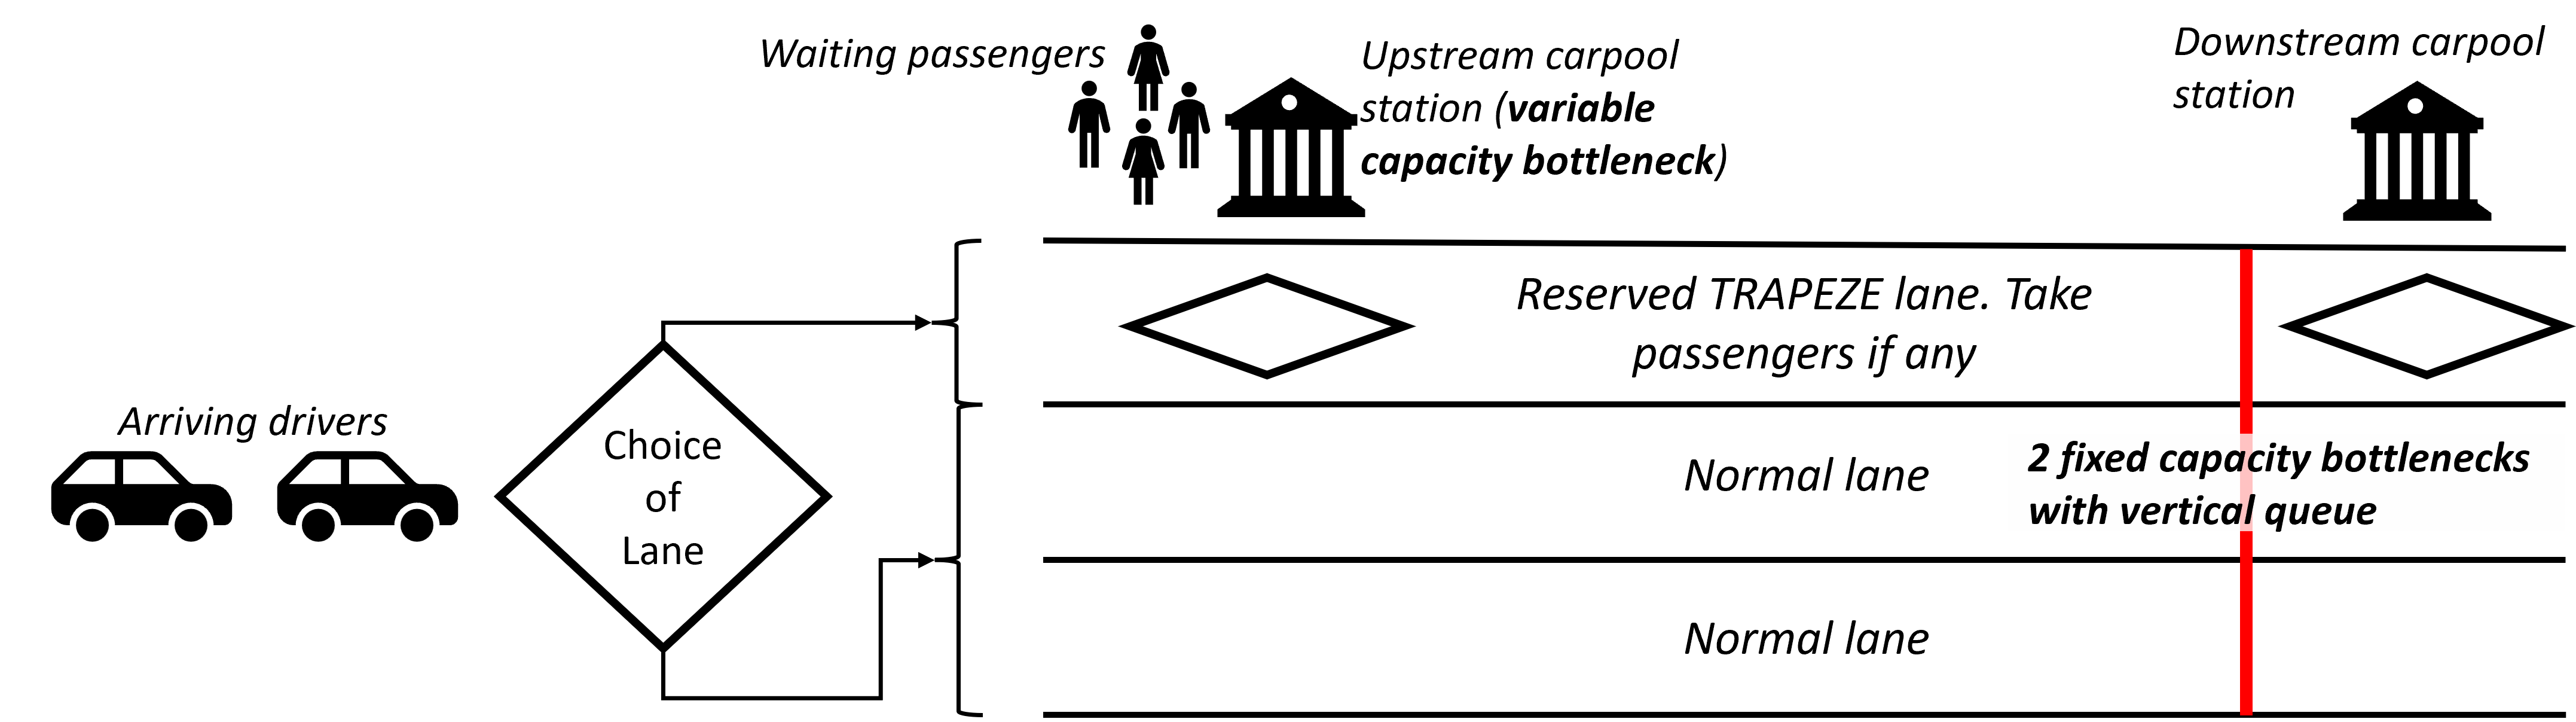
\includegraphics[width=0.85\linewidth]{images/metro_like_carpool_hov_schema.png}
    \caption{Schema of the TRAPEZE inspired HOV set-up}
    \label{figure:metro_like_carpool_hov_schema}
\end{figure}

In a bottleneck fashion, the highway has a capacity $s$ (not to be mistaken for the subscript of solo-drivers). $\varphi$ denotes the share of the reserved capacity. \acrshort{tl} hence has a capacity of $\varphi s$ and \acrshort{gpl} a capacity of $(1-\varphi)s$. Denoting $T_f$ the free-flow travel time (common between the two lanes), $T_s(t)$ and $T_d(t)$ the travel time of a driver departing at $t$ on the \acrshort{gpl} and the \acrshort{tl} respectively, we can define $T^{\nu}_s(t)$ and $T^{\nu}_d(t)$ the respective times lost in congestion as $T^{\nu}_i(t) = T_i(t) - T_f$ where $i$ is either $s$ or $d$. We suppose that congestion occurs vertically right before the downstream station. Then, defining $r_s (t)$ and $r_d (t)$ as the respective incoming flows of solo-drivers and carpooling drivers at the beginning of the road (which is not disturbed by congestion due to the vertical queue hypothesis), and given any set of initial conditions $T^{\nu}_i(\bar{t}_i) \geq 0$, $T^{\nu}_i$ are uniquely defined by the differential equations:

\begin{equation}
    \frac{d T^{\nu}_i(t)}{dt} s_i = \left\{
    \begin{array}{lr}
        r_i (t) - s_i & \text{if } T^{\nu}_i(t) > 0\\
        \max (0, r_i (t) - s_i) & \text{if } T^{\nu}_i(t) = 0
    \end{array}
    \right.
\end{equation}
where $s_d = \varphi s$ and $s_s = (1-\varphi)s$.

As for the carpooling passengers at the upstream station, they can also queue at the station in a bottleneck fashion. Denoting $r_p(t)$ the departure rate of passengers (or arrival rate at the upstream station), $M$ the maximum number of passengers in vehicles without the driver (for example $M=3$ if all vehicles are small cars with 4 seats), $q^{\nu}_p(t)$ the number of passengers waiting at the station at time $t$, and given an initial condition $q^{\nu}_p(\bar{t}_p) \geq 0$, $q^{\nu}_p$ is uniquely defined by the differential equation below:

\begin{equation}
    \label{equation:passengers_queue_at_station}
    \frac{d q^{\nu}_p(t)}{dt} = \left\{
    \begin{array}{lr}
        r_p (t) - M r_d (t) & \text{if } q^{\nu}_p(t) > 0\\
        \max (0, r_p (t) - M r_d (t)) & \text{if } q^{\nu}_p(t) = 0
    \end{array}
    \right.
\end{equation}

Then, we can define $T^{\nu}_p(t)$ the time elapsed between an arrival at the upstream station at time $t$ and the departure from that station supposing a \acrfull{fifo} queuing method as:

\begin{itemize}
    \item if $q_p^{\nu}(t) = 0$, let $\Omega = \{T_p^\nu \quad \text{s.t } q_p^\nu(t + T_p^\nu) > 0\}$
    \begin{itemize}
        \item if $\Omega = \emptyset$, then $T^{\nu}_p(t) = +\infty$
        \item else $T^{\nu}_p(t) = \inf \Omega$
    \end{itemize}
    \item else $q_p^{\nu}(t) > 0$
    \begin{itemize}
        \item if there is no $T^{\nu}_p \geq 0$ such that $M \times \int_{t}^{t+T^{\nu}_p} r_d(t) dt \geq q_p^{\nu}(t)$, then $T^{\nu}_p(t) = +\infty$
        \item else, $T^{\nu}_p(t)$ is the smallest $T^{\nu}_p \geq 0$ such that $M \times \int_{t}^{t + T^{\nu}_p} r_d(t') dt' \geq q_p^{\nu}(t)$
    \end{itemize}
\end{itemize}

Finally, we define the travel time of a carpooling passenger arriving at the station at $t$ as the sum of the time spent waiting at the station and the travel time, namely $T_p(t) = T^{\nu}_p(t) + T_d(t + T^{\nu}_p(t)) = T^{\nu}_p(t) + T^{\nu}_d(t + T^{\nu}_p(t)) + T_f$.


\subsection{Population and costs}


We suppose that we have a fixed demand of $N$ commuters. All of these commuters wish to arrive at the same desired arrival time $t^*$. By choosing a mode $i\ \in \left\{ s, d, p \right\}$ and a departure time $t$, they experience a travel time cost $\alpha \times T_i(t)$ (which will be shortened as $\text{tt}_i$) where $\alpha$ is the shadow value of travel time. They also experience a delay cost $\max [\beta \times (t^* - (t + T_i(t))), \gamma \times ((t + T_i(t)) - t^*)]$ (which will be shortened as $\text{sched}_i(t)$) where $\beta$ and $\gamma$ are the respective shadow values of time early and late. As usual in bottleneck formulations, we suppose $0 < \beta < \alpha$ and $0 < \gamma$. 

Every driver, either $s$ or $d$, also experiences a cost $f$ to operate their car that represents the cost of energy (hence the letter $f$ for ``fuel'') but also wear and tear costs, insurance cost, repair costs... All externalities due to car use but congestion are represented by the cost $E$ (for ``externality''). These are not experienced by drivers when choosing their mode, but are included in social cost functions. This could represent the sum of safety, air quality and environmental externalities for example.

The drivers of the reserved lanes are supposed to be insensitive to the expected probability of having passengers. By proposing their seats (whether there are passengers seated on them or not), they experience the potentially negative inconvenience cost $\overline{\Delta_d}$ \footnote{The fact that $\overline{\Delta_d}$ is independent of the probability of the driver to embark passengers is unrealistic. If it were certain that no commuter ever chooses the passenger mode, drivers would be indifferent between offering their seats or not for they would know that their offer is nothing but virtual. We will see however that this unrealistic case only occurs with unrealistic values, and that this simplifying hypothesis is not much of a problem when interpreting the results.}.

Similarly, carpooling passengers experience an inconvenience cost $\Delta _p$. However, opposite to carpooling driver inconvenience cost, this cost is distributed in the population\footnote{This choice of a distributed $\Delta_p$ is highly supported by literature. \alert{make citations of literature review again}.} according to the cumulative distribution function $F$. For example, there are $N \times F(\Delta _p ^0)$ commuters whose $\Delta _p$ value is lower than $\Delta _p ^0$.

While it seems logical to think that inconvenience costs of drivers and passengers would be both distributed, we had to focus on only one distribution to keep the model tractable. The choice of passengers supported by empirical literature \parencites{le_goff_are_2022, olave-cruz_does_2025} that tend to say that passengers might be the scarce resource of carpooling in a relative abundance of drivers. Moreover, once driving, sharing seats or not does not change the time needed to reach the highway entry (first leg of the trip) or the final destination (final leg of the trip). This is not the case for passengers who need to get to the departing station and to link the end station to their final destination. The difference between being passenger or not is therefore expected to have much stronger variations among individuals than between sharing seats or not as a driver.

We also suppose that the values of $\Delta _p$ are bounded and that these bounds are reached. That is to say that there is at least one commuter whose passenger inconvenience cost is $\Delta _p ^{\text{min}}$ and $\Delta _p^{\text{min}} \leq \Delta _p$ for all other commuters. Similarly, there is at least one commuter whose passenger inconvenience cost is $\Delta _p ^{\text{max}}$ and $\Delta _p^{\text{max}} \geq \Delta _p$ for all other commuters. We also suppose that:
\begin{itemize}
    \item $F$ is continuous, differentiable, and strictly increasing,
    \item The density function which is the derivative of $F$ and denoted $F'$ is well-defined, continuous and positive.
    \item $F^{-1} := [0, 1] \longrightarrow [\Delta_p^{\text{min}}, \Delta_p^{\text{max}}]$ the invert of $F$ is well-defined, continuous and differentiable.
    \item The derivative of $F^{-1}$, $(F^{-1})^{'} = \frac{1}{F'\circ F^{-1}}$ is well-defined, positive and continuous.
\end{itemize}
\alert{Could it be shortened?}

Finally, carpooling drivers and passengers both have to pay a (potentially negative) fare for choosing their mode. This fare can be time-dependent. A carpooler choosing mode $i \in \left\{ p, d \right\}$ and departing at time $t$ would have to pay a fare $\rho _i (t)$.

To summarize, a commuter departing at time $t$ with a given $\Delta _p$ value will experience the following costs depending on the mode she chooses:

\begin{equation}
\left\{
\begin{array}{l}
    c_s(t) = \text{tt}_s(t) + \text{sched}_s(t) + f\\
    c_d(t) = \text{tt}_d(t) + \text{sched}_d(t) + f + \overline{\Delta _d} + \rho _d (t)\\
    c_p(t) = \text{tt}_p(t) + \text{sched}_p(t) + \Delta _p + \rho _p (t)
\end{array}
\right.
\end{equation}
% introducing an equation is introducing a bias. don’t forget to say it.

Her contribution to social cost will be:
\begin{equation}
    \left\{
    \begin{array}{l}
        sc_s(t) = c_s(t) + E\\
        sc_d(t) = c_d(t) + E - \rho _d (t)\\
        sc_p(t) = c_p(t) - \rho _p(t)
    \end{array}
    \right.
\end{equation}

The organizer of the carpooling service will experience a profit (potentially negative) of:

\begin{equation}
    \int_{\text{time}} (r_p(t) \rho _p(t) + r_d(t) \rho _d(t)) dt
\end{equation}

Without loss of generality, we can suppose that $T_f = 0$ and that there is no queue before the first commuter arrives, either on the road or at the upstream carpooling station.


\section{Equilibria for time-independent fares} % Il faut justifier que l’on commence dans un système sans optimum global.

This paper aims to understand the behavior of a TRAPEZE system as it might be realistically implemented. In the view of the authors, it is unlikely that fares and tolls vary rapidly in the first implementations of such a system (tolls do not vary with time in France and the TRAPEZE project seeks to find a pilot implementation in France at the time of writing). We therefore focus on time-independent fare policies. We hence rewrite $\rho _d(t)$ as $\rho _d$ and $\rho _p(t)$ as $\rho _p$. To reach a first best solution, Appendix \ref{appendix_sec:extension_first_best} explores time-dependent fare policies.

\subsection{Condition for equilibrium existence}

Before understanding under which conditions an equilibrium may exist under many circumstances, we define the notion of ``feasible modal split'' with the intuitive definition below:

\begin{definition}[Feasible modal split]
    For a given capacity sharing policy $\varphi$, a triplet of real numbers $(N_s, N_d, N_p)$ is said to be a ``feasible modal split'' if:
    \begin{itemize}
        \item $N_i \geq 0$ for all $i\in \{s, d, p\}$
        \item $N_s + N_d + N_p = N$
        \item $N_p \leq MN_d$
        \item $N_s > 0 \implies \varphi < 1$
        \item $N_d > 0 \implies \varphi > 0$
    \end{itemize}
\end{definition}

\begin{proposition}
    \label{proposition:equilibrium_implies_feasible_modal_split}
    If an equilibrium exists, it necessarily defines a ``feasible modal split''.
    
    Said otherwise, if the $N$ commuters split among the three modes ($s$, $d$ or $p$) such that none has a strict interest to change its departure time nor his mode, then the thereby formed triplet $(N_s, N_d, N_p)$ satisfies the definition of ``feasible modal split''.
\end{proposition}

\begin{proof}
    See Appendix \ref{proof:equilibrium_implies_feasible_modal_split}.
\end{proof}

We further add the definition of a ``classical bottleneck’s departure rate'' which follows the most classical results of the bottleneck literature:

\begin{definition}[Classical bottleneck’s departure rate]
    $N_i$ commuters choosing mode $i$ on a road with capacity $s_i$ is said to arrive according to a ``classical bottleneck’s departure rate'' if:

    \begin{equation}
        r_i(t) = \left\{
        \begin{array}{lr}
            0 & \text{if } t<t_i^0\\
            s_i\left( 1 + \frac{\beta}{\alpha - \beta} \right) & \text{if } t_i^0 \leq t < \tilde{t}_i\\
            s_i\left( 1 - \frac{\gamma}{\alpha + \gamma} \right) & \text{if } \tilde{t}_i \leq t \leq t_i^1\\
            0 & \text{if } t_i^1 < t
        \end{array}
        \right.
        \end{equation}
        where
        
        \begin{equation}
        \left\{
        \begin{array}{l}
            t_i^0 = t^* - \frac{N_i}{s_i} \times \frac{\gamma}{\beta + \gamma}\\
            \tilde{t}_i = t^* - \frac{N_i}{s_i} \times \frac{\beta \gamma}{\alpha(\beta + \gamma)}\\
            t_i^1 = t^* + \frac{N_i}{s_i} \times \frac{\beta}{\beta + \gamma}
        \end{array}
        \right.
    \end{equation}
\end{definition}

This definition finally gives us the following proposition about how drivers will spread their departure times in the case of equilibrium:

\begin{proposition}
\label{proposition:equilibrium_implies_classical_bottleneck_departure_rate}
    In the case of equilibrium:
    \begin{itemize}
        \item If $N_s > 0$ (which implies $s_s = (1 - \varphi)s > 0$), then solo-drivers spread across time according to a ``classical bottleneck’s departure rate'' with road capacity $(1 - \varphi ) s$.
        \item If $N_d > 0$ (which implies $s_d = \varphi s > 0$), then carpooling drivers spread across time according to a ``classical bottleneck’s departure rate'' with road capacity $\varphi s$.
        \item If $N_p > 0$ (which implies $N_d \geq N_p / M > 0$ which implies carpooling drivers’ departure times spread according to a ``classical bottleneck’s departure rate''), then the departure rate function of passengers $r_p(t)$ should satisfy:\begin{itemize}
            \item $0 \leq r_p(t) \leq M r_d(t)$ for all $t\in \mathbb{R}$
            \item $N_p = \int_{t_d^0}^{t_d^1} r_p(t) dt$
        \end{itemize}
    \end{itemize}
\end{proposition}

\begin{proof}
    See Appendix \ref{proof:equilibrium_implies_classical_bottleneck_departure_rate}.
\end{proof}

\begin{remark} \begin{itemize}
    \item If $N_p = 0$, then the only departure rate available is $r_p = 0$.
    \item If $0 < N_p < MN_d$, then there are an infinity of $r_p$ functions satisfying the conditions of Proposition \ref{proposition:equilibrium_implies_classical_bottleneck_departure_rate}.
    \item If $N_p = MN_d$, then the only $r_p$ function that satisfies the conditions of Proposition \ref{proposition:equilibrium_implies_classical_bottleneck_departure_rate} is $r_p(t) = Mr_d(t)$. Said otherwise, passengers departure times spread according to a ``classical bottleneck’s departure rate'' with road capacity $M \varphi s$.

    \end{itemize}
\end{remark}

Defining $\delta = \frac{\beta\gamma}{\beta + \gamma}$, the cost incurred by a traveler of each mode immediately follows:

\begin{proposition}
    \label{proposition:equilibrium_modal_costs}
    At equilibrium, the cost incurred by a commuter with passenger inconvenience cost $\Delta_p$ choosing mode $i\in \{s, d, p\}$ given a fare policy $(\rho_d, \rho_p)$ and a capacity sharing policy $\varphi$ is:
    \begin{equation}
        \left\{
        \begin{array}{ll}
            c_s(N_s) = \frac{\delta N_s}{(1-\varphi )s} + f & \text{($\varphi < 1$, otherwise the mode cannot be chosen)}\\
            c_d(N_d) = \frac{\delta N_d}{\varphi s} + f + \overline{\Delta _d} + \rho _d & \text{($\varphi > 0$, otherwise the mode cannot be chosen)}\\
            c_p(N_d, \Delta _p) = \frac{\delta N_d}{\varphi s} + \Delta _p + \rho _p & \text{($\varphi > 0$, otherwise the mode cannot be chosen)}
        \end{array} 
        \right.
    \end{equation}
    which is independent of departure time $t$.
\end{proposition}

\begin{proof}
See Appendix \ref{proof:equilibrium_modal_costs}.
\end{proof}

Then, following the idea of \cite{konishi_carpooling_2010}, we have the following property on equilibria:

\begin{proposition}
\label{proposition:passengers_self_select_as_smallest_inconvenience_cost}
    At equilibrium, if there are some carpooling passengers ($N_p > 0$), then these passengers are the $N_p$ commuters with the lowest value of $\Delta_p$. Said otherwise, all commuters with a $\Delta_p$ value lower than $\Delta_p^{\text{switch}} = F^{-1}\left(\frac{N_p}{N}\right)$ are passengers, and other commuters are one of the $N_d + N_s$ drivers.
\end{proposition}

\begin{proof}
    See Appendix \ref{proof:passengers_self_select_as_smallest_inconvenience_cost}.
\end{proof}

\begin{remark}
    This interesting proposition could also be rephrased as ``At equilibrium, commuters self-select as passengers in a way that optimize social cost.''.

    The system therefore seems to function well in that matter.
\end{remark}

Finally, it is possible to define the conditions of existence of an equilibrium:

\begin{proposition}
\label{proposition:equilibrium_existence_conditions}
    \begin{itemize}
        \item If $\varphi = 0$, the only modal split at equilibrium is $N_s = N$ and $N_p = N_d = 0$.
        \item If $\varphi = 1$, there exists an equilibrium if and only if one and only one of the following conditions is satisfied:
        \begin{itemize}
            \item \begin{equation} \label{equation:phi0_condD} c_d(N) \leq c_p(N, \Delta_p^{\text{min}}) \end{equation} (everybody drives while sharing their seats, denoted ``D'')
            \item exclusive or \begin{equation} \label{equation:phi0_condDPmax} c_d\left(\frac{N}{M + 1} \right) = c_p\left(\frac{N}{M + 1}, F^{-1}\left(\frac{M}{M + 1}\right)\right) \end{equation} (maximum carpooling capacity is reached, denoted ``DPmax'')
            \item exclusive or \begin{equation} \label{equation:phi0_condDP} \exists N_p \in \left]0, \frac{M}{M+1}\right[ \quad \text{s.t. } c_d(N - N_p ) = c_p\left(N - N_p, F^{-1}\left(\frac{N_p}{N}\right)\right)\end{equation}
        \end{itemize}
        This is equivalent to saying that there is no equilibrium if and only if $F^{-1}\left(\frac{M}{M + 1}\right) + \rho_p < f + \overline{\Delta_d} + \rho_d$.
        \item If $0 < \varphi < 1$, there exists an equilibrium if and only if one and only one of the following conditions is satisfied:
        \begin{itemize}
            \item \begin{equation} \label{equation:phiint_condS} c_d(0) \geq c_s(N) \leq c_p(0, \Delta_p^{\text{min}})\end{equation} (everybody drives solo, denoted ``S''),
            \item exclusive or \begin{equation} \label{equation:phiint_condD} c_s(0) \geq c_d(N) \leq c_p(N, \Delta_p^{\text{min}})\end{equation} (everybody drives on the \acrshort{tl}, denoted ``D''),
            \item exclusive or \begin{equation} \label{equation:phiint_condDPmax} c_s(0) \geq c_d\left(\frac{N}{M + 1} \right) = c_p\left(\frac{N}{M + 1}, F^{-1}\left(\frac{M}{M + 1}\right) \right) \end{equation} (everybody carpools and the car capacity is reached, denoted ``DPmax''),
            \item exclusive or \begin{equation} \label{equation:phiint_condDP} \exists N_d \in \left] \frac{N}{M + 1}, N \right[ \quad \text{s.t. }c_s(0) \geq c_d(N_d) = c_p \left( N_d, F^{-1} \left( \frac{N - N_d}{N} \right) \right) \end{equation} (everybody carpools and the car capacity is not reached, denoted ``DP''),
            \item exclusive or \begin{equation} \label{equation:phiint_condSD} \exists N_s \in ]0, N[ \quad \text{s.t. } c_s(N_s) = c_d(N - N_s) \leq c_p(N - N_s, \Delta_p^{\text{min}}) \end{equation} (some drive solo and some share their seats without passengers, denoted ``SD''),
            \item exclusive or \begin{equation} \label{equation:phiint_condSDPmax} \exists N_s \in ]0, N[ \quad \text{s.t. } c_s(N_s) = c_d\left(\frac{N - N_s}{M + 1}\right) = c_p\left(\frac{N - N_s}{M + 1}, F^{-1} \left( \frac{N - N_s}{N}\times \frac{M}{M + 1} \right)\right) \end{equation} (some drive solo and some carpool while filling the carpooling vehicles up to their capacity, denoted ``SDPmax''),
            \item exclusive or \begin{multline} \label{equation:phiint_condSDP} \exists N_s \in ]0, N[ \text{ and } N_d \in \left] \frac{N - N_s}{M + 1}, N - N_s\right[ \\ \text{s.t. } c_s(N_s) = c_d(N_d) = c_p\left(N_d, F^{-1}\left( \frac{N - N_s - N_d}{N} \right)\right) \end{multline} (all modes without reaching vehicle capacity, denoted ``SDP'').
        \end{itemize}
        This is equivalent to saying that there is no equilibrium if and only if:
        \begin{itemize}
            \item \begin{equation*}
                \left\{
                \begin{array}{l}
                    \rho _d \leq - \frac{\delta}{\varphi s}\times \frac{N}{M+1} - \overline{\Delta _d}\\
                    \rho _p - \rho _d < f + \overline{\Delta _d} - F^{-1}\left(\frac{M}{M + 1}\right)
                \end{array}
                \right.
            \end{equation*}
            \item or \begin{equation*}
                \left\{
                \begin{array}{l}
                    -\frac{\delta}{\varphi s}\times \frac{N}{M+1} - \overline{\Delta _d} < \rho _d < \frac{\delta N}{(1-\varphi ) s} - \overline{\Delta _d}\\
                    \rho _p - \rho _d < f + \overline{\Delta _d} - F^{-1}\left( \frac{M}{(M+1)N} \times \left( N - \frac{\rho_d + \frac{\delta}{\varphi s}\times \frac{N}{M+1} + \overline{\Delta _d}}{\frac{\delta}{s}\times \left( \frac{1}{1-\varphi} + \frac{1}{\varphi (M+1)} \right)} \right)\right)
                \end{array}
                \right.
        \end{equation*}
        \end{itemize}
    \end{itemize}
    In all cases, for a given capacity sharing policy $\varphi$ and a given fare policy $(\rho_d, \rho_p)$, the modal split is common to all equilibrium and it is only the departure rate of passengers that may differ between equilibria\footnote{as well as which commuters departs when since they are all indifferent to that variable in such an equilibrium}. If $N_p \in [0, MN_d]$, the departure rate is unique, otherwise it is non unique.
\end{proposition}

\begin{proof}
    See Appendix \ref{proof:equilibrium_existence_conditions}.
\end{proof}

Some characterizations of equilibria as well as some illustrations are provided in the next subsection (Subsection \ref{subsection:characteristics_of_equilibria}).

Another very interesting proposition about equilibria is as follows:

\begin{proposition}
\label{proposition:policiy_existence_from_almost_feasible_modal_split}
    For any triplet $(N_s, N_d, N_p)$ satisfying
    \begin{itemize}
        \item $N_i \geq 0$ for all $i\in \{s, d, p\}$
        \item $N_s + N_d + N_p = N$
        \item $N_p \leq MN_d$ 
    \end{itemize}
    there exists a capacity sharing policy $\varphi$ and a fare policy $(\rho_d, \rho_p)$ (non-necessarily unique) such that $(N_s, N_d, N_p)$ is a feasible modal split that is an equilibrium under these policies.
\end{proposition}

\begin{proof}
    See Appendix \ref{proof:policiy_existence_from_almost_feasible_modal_split}.
\end{proof}

\alert{Guillaume: Selon le journal que l’on vise, on pourrait avoir une contribution méthodologique poussée comme ici (Part B) ou être encore plus rapide (JUE).}

\subsection{Description of equilibria}
\label{subsection:characteristics_of_equilibria}

This subsection provides some illustrations and understandings about the equilibrium described by the series of propositions in the previous subsection. The first subsubsection shows the time departure rates of equilibria, the second maps how modal splits can be chosen with the help of policies, the third elaborates symbolically the way this paper builds on state of the art bottleneck carpooling literature and proposes significant methodological improvements, and the last subsubsection draws further conclusions from Propositions \ref{proposition:equilibrium_existence_conditions} and \ref{proposition:policiy_existence_from_almost_feasible_modal_split}, thus introducing the next section about optimal policies.

\subsubsection{Description of departure and arrival rates at equilibrium}

As seen in Proposition \ref{proposition:equilibrium_implies_classical_bottleneck_departure_rate}, with time-independent fare policies, solo-drivers’ and carpooling drivers’ departure rates are those of classical bottleneck’s literature, and those of carpooling passengers are more flexible, though constrained in their form.

To visualize these features, Figure \ref{figure:arrival_rates} provides an illustration of the three categories of equilibria for $\varphi = 1$, namely D, DP and DPmax, as described in Proposition \ref{proposition:equilibrium_existence_conditions}.

\begin{figure}
\begin{center}
    \begin{subfigure}{.49\textwidth}
    \begin{center}
        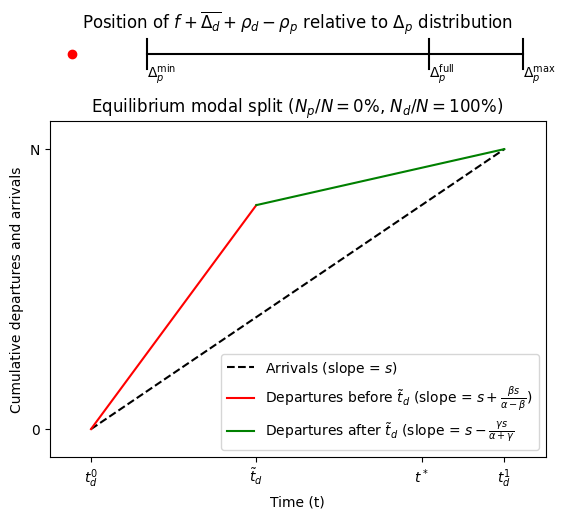
\includegraphics[width=\textwidth]{images/arrivals1.png}
        \caption{No passenger (case D): equilibrium is unique}
        \label{subfigure:arrival_rates_no_passenger}
    \end{center}
    \end{subfigure}% this comment has to be here to avoid vertical stacking of figures
    \hfill
    \begin{subfigure}{.49\textwidth}
    \begin{center}
        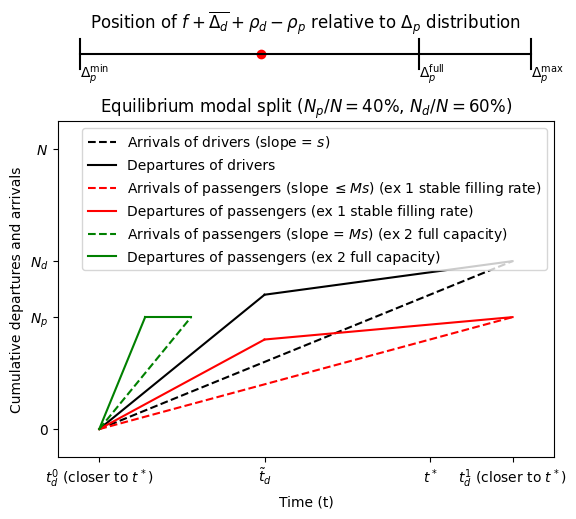
\includegraphics[width=\textwidth]{images/arrivals2.png}
        \caption{Partial utilization of car capacity (case DP): equilibrium is unique for drivers and infinite for passengers}
        \label{subfigure:arrival_rates_interior}
    \end{center}
    \end{subfigure}% this comment has to be here to avoid vertical stacking of figures
    \hfill
    \begin{subfigure}{.49\textwidth}
    \begin{center}
        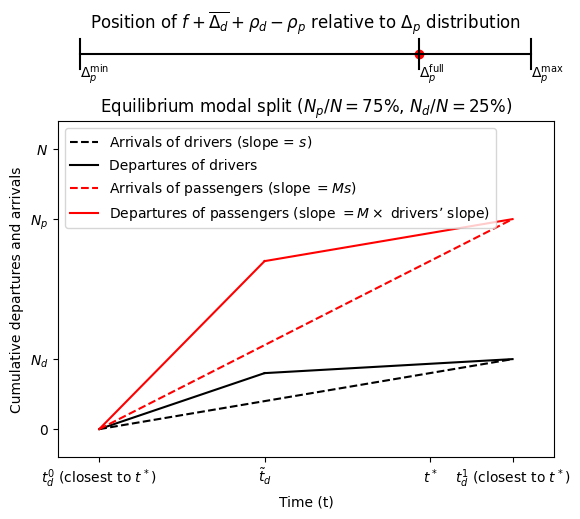
\includegraphics[width=\textwidth]{images/arrivals3.png}
        \caption{Full utilization of car capacity (case DPmax): equilibrium is unique for drivers and passengers}
        \label{subfigure:arrival_rates_max_capacity}
    \end{center}
    \end{subfigure}

\caption{Departure and arrival rates of drivers and passengers for the three equilibrium regimes of $\varphi = 1$. Dotted lines represent cumulative arrivals and solid lines cumulative departures. $M = 3$}
\label{figure:arrival_rates}
\end{center}
\end{figure}

In the absence of passengers (Figure \ref{subfigure:arrival_rates_no_passenger}, case D), which corresponds to $f + \overline{\Delta_d} + \rho_d \leq \Delta_p^{\text{min}} + \rho_p$, arrival rate of commuters follows the maximum outflow rate of the bottleneck: $s$. However, the departure rate of drivers differs from bottleneck’s capacity at equilibrium and creates a useless lost time in congestion which equals the irreducible delay costs imposed by the bounded capacity of the bottleneck (see \alert{citation} for more details).

As passengers replace drivers ($f + \overline{\Delta_d} + \rho_d - \rho_p$ increases relative to $\Delta_p$ distribution), drivers still follow a classical bottleneck departure rates but are less numerous (drivers with $\Delta_p$ values lower than $f + \overline{\Delta_d} + \rho_d - \rho_p$ switched to passengers). Therefore, one can notice in Figure \ref{subfigure:arrival_rates_interior} (case DP) that $N_d < N$ in the vertical axis. Also, the slopes for drivers’ departure rate function are the same, which shows that the vertical axis has been zoomed in around $t^*$ (although $t^*$ did not move, nor the relative positions of $t_d^0, \tilde{t}_d$ and $t_d^1$ to $t^*$, these three values are closer to $t^*$ in Figure \ref{subfigure:arrival_rates_interior} than in Figure \ref{subfigure:arrival_rates_no_passenger}). As for passengers, there is no single arrival rate that is a solution. On this figure, only two of them are represented:\begin{itemize}
    \item in green, passengers maximize the car usage of all the first drivers while letting other drivers with empty seats (since $M = 3$ in Figure \ref{figure:arrival_rates}, the first slope of passengers’ departure is exactly three times that of drivers’);
    \item in red, passengers choose a uniform filling rate for all drivers’ vehicles.
\end{itemize}
But these are only examples, some passengers could arbitrarily decide to change their departure time (for the same cost). As long as all passengers depart within the time frame of drivers’ departures, and as long as $r_p(t) \leq r_d(t)$ at all time, this would be an equilibrium. All these departure rates of passengers result in the same cost for passengers and the same social costs for the system.

Further increasing the number of passengers (at the expense of drivers),  the maximum capacity of drivers’ cars is reached ($f + \overline{\Delta_d} + \rho_d - \rho_p = \Delta_p^{\text{full}} := F^{-1}\left( \frac{M}{M + 1} \right)$). While drivers still depart according to ``classical bottleneck’s departure rates'' (x-axis is further zoomed in), in order not to queue at the upstream station, passengers have no choice but to strictly follow drivers’ departure rates (with a loading factor of $M$) as illustrated in Figure \ref{subfigure:arrival_rates_max_capacity} with $M = 3$.

Increasing $f + \overline{\Delta_d} + \rho_d$ beyond $\Delta_p^{\text{full}} + \rho_p$ would yet suppress the existence of economic equilibrium (some drivers would have a strict interest to switch to passenger and depart before the first passengers if $N_p \leq MN_d$, and some passengers would wait endlessly without drivers at the upstream station if $N_p > MN_d$). No equilibrium can therefore be represented.



\subsubsection{Managing equilibrium through policies}

Proposition \ref{proposition:equilibrium_existence_conditions} says that, for each capacity sharing policy $\varphi \in [0, 1]$, whatever the fare policy $(\rho_d, \rho_p)$, either their is a unique modal split that is an equilibrium falling in one and only one equilibrium category (S, D, DP, DPmax, SD, SDP, SDPmax), or there is no equilibrium at all.

It is thus possible to map equilibria according to policies. Figure \ref{figure:equilibrium_phase_diagram} does it for some value $\varphi \in ]0, 1[$ (the map is trivial for $\varphi = 0$ and upper parts of Figure \ref{figure:arrival_rates}’s subfigures does it somehow for $\varphi = 1$). The arrows on the plot show to what equilibrium numbered solid lines belong. Unnumbered dotted lines are equilibrium cases on their own\footnotemark. The equations of lines are described in Appendix \ref{appendix:phase_diagram_equations}.

\footnotetext{The distribution used in this illustration is some arbitrary trapezoidal distribution (see \texttt{scipy.stats.trapezoid} (version \textit{1.15.2}) documentation on \href{https://docs.scipy.org/doc/scipy-1.15.2/reference/generated/scipy.stats.trapezoid.html}{https://docs.scipy.org} for documentation). Changing the shape of $F$ without changing $\Delta_p^{\text{min}}$ and $F^{-1}\left( \frac{M}{M+1} \right)$ would change the shape of lines (4) and (SDPmax) but nothing else (including the position of intersection points).}.

\begin{figure}
    \centering
    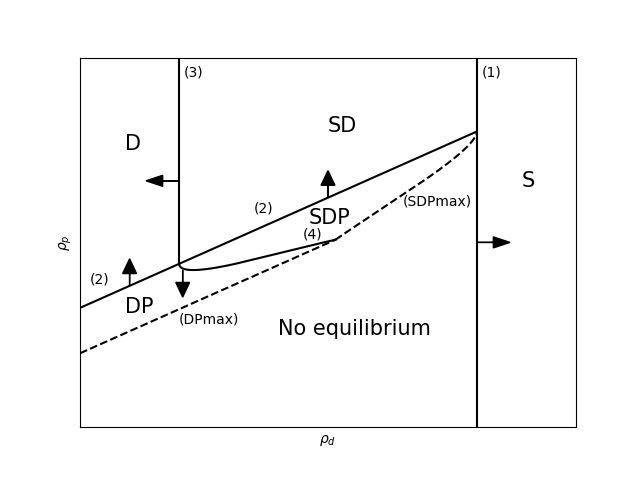
\includegraphics[width=0.5\linewidth]{images/equilibrium_phase_diagram_trapezoidal_dist.png}
    \caption{Phase diagram of equilibrium cases according to fare policies for $\varphi \in ]0, 1[$.}
    \label{figure:equilibrium_phase_diagram}
\end{figure}

\begin{remark}
    According to Proposition \ref{proposition:policiy_existence_from_almost_feasible_modal_split}, we know that given a capacity sharing policy ($\varphi \in ]0, 1[$), the function associating a fare policy with the feasible modal split that results from equilibria is a surjection..
    
    However, due to the bijectivity of $F$, we could actually prove more: for a given capacity sharing policy $\varphi \in ]0, 1[$, reducing the definition space of the function above to the SDP area (including its contour) makes it a bijection.
\end{remark}



\section{Optimal management of TRAPEZE system (fixed capacity)}
\alert{In this section, avoid cluttering properties but stick to the core message. For the moment it is a non organized enumeration of potential properties}

In this section, we describe what optimal policies look like and how they perform. If we assume that setting a policy (capacity sharing or fare) is free, and if we assume that fares are only transfers between agents, thus transparent to Social Cost, then Social Cost is only determined by modal splits. This is where Propositions \ref{proposition:equilibrium_existence_conditions} and \ref{proposition:policiy_existence_from_almost_feasible_modal_split} come to the rescue. Choosing optimal policies can simply be achieved by choosing optimal feasible modal shares and optimal capacity sharing policies. This optimization process can be done without knowledge about the corresponding fare policies to obtain these equilibria. Fare policies can be determined afterward.

For the moment we suppose that the reserved capacity is fixed to some value $\varphi$. Three cases can occur:

\subsection{\texorpdfstring{$\varphi = 0$}{varphi = 0}}

In that case, policies have no effect and equilibria are those of classical bottleneck models: social cost is $SC_{\varphi = 0} = \frac{\delta N^2}{s} + N(f + E)$ and all passengers experience a user-cost $UC = \frac{\delta N}{s} + f + E$.

The carpooling operator makes a null profit.

\subsection{\texorpdfstring{$\varphi = 1$}{varphi = 1}}

Now, all commuters are forced to participate in the TRAPEZE system and we have:

\begin{equation}
    SC_{\varphi = 1} = \frac{\delta N_d^2}{s} + \frac{\delta N_d N_p}{s} + N_d (\overline{\Delta_d} + f + E) + \int_{\Delta_p^{\text{min}}}^{F^{-1}\left( \frac{N_p}{N} \right)} \Delta_pdF
\end{equation}

Under the four constraints $N_d \geq 0$, $N_p \geq 0$, $N = N_d + N_p$ and $N_p \leq MN_d$, we find the following set of feasible modal splits minimizing $SC$:
\begin{itemize}
    \item if $\frac{\delta N}{s} + f + E + \overline{\Delta_d} \leq \Delta_p^{\text{min}}$: then $N_d = N$ and $N_p = 0$
    \item else if $\frac{\delta N}{s} + f + E + \overline{\Delta_d} \geq \Delta_p^{\text{full}}$, then $N_d = \frac{N}{M + 1}$ and $N_p = \frac{NM}{M + 1}$
    \item else, let $\Delta_p^{\text{switch}} = \frac{\delta N}{s} + f + E + \overline{\Delta_d} \in ]\Delta_p^{\text{min}}, \Delta_p^{\text{full}}[$, then $N_d = N(1 - F(\Delta_p^{\text{switch}}))$ and $N_p = F(\Delta_p^{\text{min}})$.
\end{itemize}

The usual equilibrium condition is $\rho_d - \rho_p = F^{-1}\left(\frac{N_p}{N} \right) - f - \overline{\Delta_d}$. For the interior condition, one can note that it equates $\frac{\delta N}{s} + E$, which is the sum of the congestion externality and other externalities, as usual with optimal pricing in the presence of externalities.

Also, profit is not defined since it is only the difference between the two fares that is constrained with $\varphi = 1$. The carpooling service could potentially make an infinite profit or an infinite loss.

\begin{remark}
    We have already noted that having carpooling drivers without passengers would make the setting rather unrealistic in the sense that drivers may take the wheel knowing they will not really experience their inconvenience cost.

    However, to get to such a setting, it should be the case that $\overline{\Delta_d} \leq \Delta_p^{\text{min}} - f - E - \frac{\delta N}{s}$, which has a high probability of being negative if $\Delta_p^{\text{min}}$ is not too high, especially as congestion grows big, which is the usual configuration to consider implementing lane reservation. Such a case should therefore almost never occur in reality.
\end{remark}

\subsection{\texorpdfstring{$0 < \varphi < 1$}{0 < varphi < 1}}

This time, we are trying to optimize

\begin{equation}
\label{equation:SC_interior_3vars}
    SC_{0 <\varphi<1} = \frac{\delta N_s^2}{(1 - \varphi ) s} + \frac{\delta N_d^2}{\varphi s} + \frac{\delta N_d N_p}{\varphi s} + (N_s + N_d)(f + E) + N_d\overline{\Delta_d} + \int_{\Delta_p^{\text{min}}} ^{F^{-1}\left( \frac{N_p}{N} \right)} \Delta_pdF
\end{equation}
under the usual constraints.

Noticing that $N_s = N - N_d - N_p$ and plugging this, we get:

\begin{equation}
\label{equation:SC_interior_2vars}
    SC_{0 <\varphi<1} (N_d, N_p) = \frac{\delta (N - N_d - N_p)^2}{(1 - \varphi ) s} + \frac{\delta N_d^2}{\varphi s} + \frac{\delta N_d N_p}{\varphi s} + (N - N_p)(f + E) + N_d\overline{\Delta_d} + \int_{\Delta_p^{\text{min}}} ^{F^{-1}\left( \frac{N_p}{N} \right)} \Delta_pdF
\end{equation}

The associated Lagrangian is:

\begin{equation}
\label{equation:lagrangian}
    SC(N_d, N_p) -\mu_s(N - N_p - N_d) - \mu_d N_d - \mu_p N_p - \mu_v(MN_d - N_p)
\end{equation}

Unfortunately, despite the space of feasible modal splits being a compact convex set, we cannot guaranty that this $SC$ is a convex function. To see that, note that the gradient of the objective function is:

\begin{equation*}
    \nabla_{SC} (N_d, N_p) = \begin{pmatrix}
        \frac{\delta}{s} \left( \frac{-2(N - N_d - N_p)}{1 - \varphi} + \frac{2 N_d + N_p}{\varphi} \right) + \overline{\Delta_d}\\
        \frac{\delta}{s} \left( \frac{-2(N - N_d - N_p)}{1 - \varphi} + \frac{N_d}{\varphi} \right) -f - E + F^{-1} \left( \frac{N_p}{N} \right)
    \end{pmatrix}
\end{equation*}

And then, the Hessian is:

\begin{equation*}
    H_{SC}(N_d, N_p) = \begin{pmatrix}
        \frac{2 \delta}{s} \left( \frac{1}{1 - \varphi} + \frac{1}{\varphi} \right) & \frac{\delta}{s} \left( \frac{2}{1 - \varphi} + \frac{1}{\varphi} \right)\\
        \frac{\delta}{s} \left( \frac{2}{1 - \varphi} + \frac{1}{\varphi} \right) & \frac{2\delta}{(1- \varphi )s} + \frac{1}{NF'\left(F^{-1}\left(\frac{N_p}{N} \right)\right)}
    \end{pmatrix}
\end{equation*}

Solving the second degree polynomial $\det (H_{SC}(N_d, N_p) - \lambda I)$, we find the two following eigenvalues: $\frac{A}{2} + \frac{\delta (\varphi + 1)}{s \varphi (1 - \varphi)} \pm \sqrt{\frac{A^2}{4} - \frac{A \delta}{s \varphi} + \frac{2 \delta^2 (\varphi^2 + 1)}{s^2 \varphi^2 (1 - \varphi)^2}}$ where $A = \frac{1}{NF'\left(F^{-1}\left( \frac{N_p}{N} \right) \right)} \geq 0$. The larger eigenvalue is always positive. For small values of $A$ ($F$ very steep, or all commuters have close $\Delta_p$ values), the smaller eigenvalue is negative since $1 + \varphi - \sqrt{2(1 + \varphi ^2}) \leq 0$ for $0 < \varphi < 1$. However, for big values of $A$ ($F$ is very flat, or commuters have dispersed $\Delta_p$ values), both eigen values go to infinity, making the problem convex.

When solving the Lagrangian, it is therefore needed to check the conditions of all corner solutions, and to compare all local minima of interior solutions.

Calculations are tedious and result conditions for optima are presented in Appendix \ref{appendix:optima_condition_fixed_varphi}. Appendix \ref{appendix_sec:extension_first_best} also proposes some intuitions to interpret the condition equations. To make sure that our calculations were correct, we proceeded to two different checks:
\begin{enumerate}
    \item Calculations were done for a linear approximation using the formal calculous library Sympy \parencite{meurer_sympy_2017}.
    \item We also built a solver, whose results were compared to the \texttt{shgo} solver of Scipy’s optimization sublibrary \parencite{virtanen_scipy_2020}.
\end{enumerate}
\alert{The code of these checks will be available on Github after the publication of the article but the repository is kept anonymous for the time of review}.

Having a look at the interior solution case (case SDP), using the equilibrium conditions as well as the first order conditions $\nabla_{SC} (N_d, N_p) = 0$, we find the following values for tolls:

\begin{itemize}
    \item $\rho_d = -\frac{\delta N_s}{(1 - \varphi ) s} + \frac{\delta (N_d + N_p)}{\varphi s}$
    \item $\rho_p = -\frac{\delta N_s}{(1 - \varphi )s} - E$
    \item and $\rho_p - \rho_d = -E - \frac{\delta (N_d + N_p)}{\varphi s}$
\end{itemize}
which can be interpreted as the sum of new externalities minus the avoided externalities in switching from solo-driver (respectively solo-driver and carpooling driver) to carpooling driver (respectively passenger and passenger).

%\subsection{Optimal pricing rules}
\subsection{Interesting properties}




\subsubsection{Increase of passengers with demand}

Not sure for the moment.

\subsubsection{Limits for extreme demand}

While the shape of $F$ makes it harder to properly predict the behavior of the model analytically (but we can do it computationally), no more knowledge than the value of $\Delta_p^{\text{min}}$ and $\Delta_p^{\text{full}}$, $F(f + E)$,  $\delta$, $f$, $E$, $M$ and $\varphi$ is required to anticipate what the optimal modal split will be for very low demand, and no knowledge at all for very high demand.

For low demand, we note that the Hessian is necessarily positive definite due to the small $N$ value and the bounded nature of $F'$. The minima is therefore unique, and only one case can be satisfied. Conditions of the different cases become:\begin{description}
    \item[Case D:] \begin{itemize}
        \item $\overline{\Delta_d} < 0$
        \item $f + E + \overline{\Delta_d} < \Delta_p^{\text{min}}$
    \end{itemize}
    \item[Case DPmax:]\begin{itemize}
        \item $\overline{\Delta_d} + f + E \geq \Delta_p^{\text{full}}$
        \item $\overline{\Delta_d} + M\Delta_p^{\text{full}} < M(f + E)$
    \end{itemize}
    \item[DP:]\begin{itemize}
        \item $\Delta_p^{\text{min}} \leq \overline{\Delta_d} + f + E < \Delta_p^{\text{full}}$
        \item $\Delta_d < 0$
    \end{itemize}
    \item[Case S:]\begin{itemize}
        \item $\overline{\Delta_d} > 0$
        \item $\overline{\Delta_d} + M \Delta_p^{\text{min}} > M(f + E)$
    \end{itemize}
    \item[Case SD]\begin{itemize}
        \item $\overline{\Delta_d} = 0$
        \item $\Delta_p^{\text{min}} > f + E$
    \end{itemize}
    \item[Case SDPmax]\begin{itemize}
        \item $M\Delta_p^{\text{min}} \leq M(f + E) - \overline{\Delta_d} \leq M\Delta_p^{\text{full}}$
        \item $\Delta_d > 0$ if $F(f + E) < \frac{2M\varphi}{2 + M + M\varphi}$ and $\Delta_d \geq 0$ otherwise
    \end{itemize}
    \item[Case SDP]\begin{itemize}
        \item $\Delta_d = 0$
        \item $F(f + E)\leq \frac{2M\varphi}{2 + M + M\varphi}$
    \end{itemize}
\end{description}

\begin{remark}
    Note that this case exhaustion is independent of road capacity $s$.
\end{remark}

For a given $F$ function only shifted by the variable $\Delta_p^{\text{min}}$ value, for the variable $\overline{\Delta_d}$, and for other fixed parameter values, it is possible to map what the optimal modal split will be as shown in Figure \ref{figure:optimal_phase_diagram}.

\begin{figure}
    \centering
    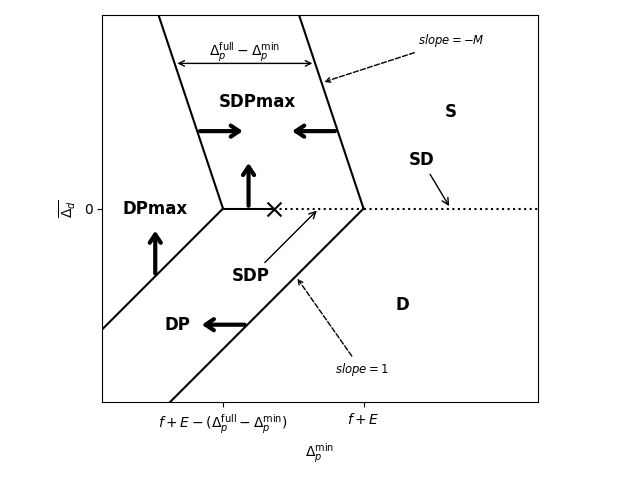
\includegraphics[width=0.5\linewidth]{images/optimal_regime_phase_diagram_Nto0.png}
    \caption{Phase diagram of optimal modal split as $N \rightarrow 0^+$ according to $\overline{\Delta_d}$ and $\Delta_p^{\text{min}}$, all other parameters (including the shape of $F$) being hold fixed. At the cross, we have $F(f + E) = \frac{2M\varphi}{2 + M + M\varphi}$.  Bold arrows indicate to what area the solid lines belong, thin solid single sided arrows indicate the name of one-dimensional areas (dotted-lines) of equilibrium types.}
    \label{figure:optimal_phase_diagram}
\end{figure}

Opposed to the very low demand, as $N$ grows to infinity, it is not hard to see that only the conditions for case SDPmax will be satisfied. Then, $\frac{N_d}{N} \rightarrow \frac{\varphi}{1 + M\varphi}$, $\frac{N_p}{N} \rightarrow \frac{M\varphi}{1 + M\varphi}$ and $\frac{N_s}{N} \rightarrow \frac{1 - \varphi}{1 + M\varphi}$.

In that case, we also have the following property (to check numerically):

\begin{proposition}
\label{proposition:lim_per_person_profit_N_big_phi_fixed}
    As demand goes to infinity, profit per user goes to the following limit:

    \begin{equation*}
        \lim_{N\rightarrow+\infty} \frac{\Pi}{N}= \frac{\varphi}{2(1 + M\varphi)} \left[  -\overline{\Delta_d} + M\left( -F^{-1} \left( \frac{M\varphi}{1 + M\varphi} \right) +f - E \right) \right]
    \end{equation*}
    as long as the within bracket term is not null.

    Said otherwise, it is possible to predict the sign of profit based on the sign of the within bracket term
\end{proposition}

\begin{proof}
    See Appendix \ref{proof:lim_per_person_profit_N_big_phi_fixed}.
\end{proof}

The consequences of Proposition \ref{proposition:lim_per_person_profit_N_big_phi_fixed} is intuitive: 
\begin{enumerate}
    \item the more reluctant commuters are toward carpooling (high values of $\overline{\Delta_d}$ and $F^{-1}$), the more carpooling needs to be subsided;
    \item the higher the other externalities $E$, the more carpooling needs to be subsided (under untolled alternative and inelastic demand);
    \item and the higher the car operation price, the more carpooling occurs naturally, and the more profit can be made by the TRAPEZE system.
\end{enumerate}

What is less intuitive however is that the \acrshort{vot} to capacity ratio ($\frac{\delta}{s}$) is unrelated to these trends.

\subsubsection{Non-extreme demand}

Doing some comparative statics, it is possible to find some more intuitive properties:

\begin{proposition}
    \label{proposition:intuitive_comparative_statics}
    Doing …
\end{proposition}

\subsubsection{More expensive environmental costs leads to more carpooling without natural incentive, and thus to more subsidy}
\subsubsection{Forcing the system to break-even}
\subsubsection{impact of vot}
\subsubsection{Reduction of interior solutions with endogenous reserved capacity}
\subsubsection{Full-utilization of capacity?}
\subsubsection{Some noteworthy model behaviors}
    \begin{itemize}
        \item Non monotonous
        \item Non continuous
        \item Multiple regimes
        \item Close regimes with very different financial outcomes (opportunity cost of public funds)
    \end{itemize}

\subsection{condition for making profit}

\section{Numerical analysis}

\alert{Find a real-world example.}

\section{Discussions, limits and further works}
\label{section:discussions_and_limits}

\begin{itemize}
    \item Bottleneck
    \item Multiple cross-distributions
    \item Normal carpooling lane comparison
    \item More modal distribution
    \item Optimizing profit?
    \item Demand elasticity and profitability with one more toll for solo-drivers.
    \item Decentralizing congestion
    \item Comparison with normal lanes
    \item Not everybody has a car
    \item rebound effect
\end{itemize}

\section{Conclusions}

\section{References}

\printbibliography

\part{Appendices}

\appendix

\section{Extension: endogenization of shared capacity}
\subsection{Set-up}
\subsection{Properties}
\subsection{Numerical analysis}

\section{Extension: First-best optimum (removing congestion)}
\label{appendix_sec:extension_first_best}
\alert{Should we remove congestion everywhere or not}

\section{Proofs}

\subsection{Proof of Proposition \ref{proposition:equilibrium_implies_feasible_modal_split}}
\label{proof:equilibrium_implies_feasible_modal_split}

For the two first conditions ($N_i \geq 0$ for all $i \in \{s, d, p\}$ and $N_s + N_d + N_p = N$), it simply follows the set-up: there is no negative individual and they must all choose one mode.

For the condition $N_p \leq MN_d$, suppose it were not the case. Then, at least one passenger could never get into any car, and therefore incur a cost of $+\infty$. This passenger would have a strict interest in changing her modal choice and such a situation could not be an equilibrium.

Similar reasonings lead to the two last conditions ($N_s > 0 \implies \varphi < 1$ and $N_d > 0 \implies \varphi > 0$). \qed

\subsection{Proof of Proposition \ref{proposition:equilibrium_implies_classical_bottleneck_departure_rate}}
\label{proof:equilibrium_implies_classical_bottleneck_departure_rate}

For solo-drivers and carpooling drivers, this is just the direct application of \alert{make citation}.

For passengers with respective $\Delta_p$ values and respective $t$ departure times, their respective incurred generalized costs are $T_p^{\nu}(t) + \frac{\delta N_d}{\varphi s} + \Delta_p + \rho_p$, where $\delta = \frac{\beta\gamma}{\beta + \gamma}$.

But whatever the passenger departure rate function $r_p(t)$, there exists at least one time at which $T_p^\nu = 0$, namely $t_d^1$ (if not, then one passenger would experience an infinite waiting cost). Therefore, if it were not the case that all passengers experience $T_p^\nu(t) = 0$, these passengers would have a strict interest in changing their departure time and it could not be an equilibrium.

Finally $T_p^\nu(t) = 0$ at all passengers’ departure times leads to $q_p^\nu(t) = 0$ at all time. Equation \ref{equation:passengers_queue_at_station} gives the first of the two conditions on passenger departure rate functions. The second condition simply says that all passengers should depart, neither more nor less.\qed

\subsection{Proof of Proposition \ref{proposition:equilibrium_modal_costs}}
\label{proof:equilibrium_modal_costs}

For solo-drivers and carpooling drivers, it immediately follows from Proposition \ref{proposition:equilibrium_implies_classical_bottleneck_departure_rate} and classical bottleneck’s literature (see \alert{make citation} for proper demonstration).
    
For passengers, we have seen this in the proof of Proposition \ref{proposition:equilibrium_implies_classical_bottleneck_departure_rate} (Appendix \ref{proof:equilibrium_implies_classical_bottleneck_departure_rate}).\qed

\subsection{Proof of Proposition \ref{proposition:passengers_self_select_as_smallest_inconvenience_cost}}
\label{proof:passengers_self_select_as_smallest_inconvenience_cost}

From Proposition \ref{proposition:equilibrium_modal_costs}, it immediately follows that if a commuter with passenger inconvenience cost $\Delta_p^0$ chooses to be passenger (meaning $c_p(N_d, \Delta_p^0) \leq c_d(N_d)$ (and $c_p(N_d, \Delta_p^0) \leq c_s(N_s)$ if $\varphi < 1$)), so would all commuters with $\Delta_p < \Delta_p^0$. And hence comes the proposition. \qed

\subsection{Proof of Proposition \ref{proposition:equilibrium_existence_conditions}}
\label{proof:equilibrium_existence_conditions}

\subsubsection{Case \texorpdfstring{$\varphi = 0$}{phi = 0}}
Due to Proposition \ref{proposition:equilibrium_implies_feasible_modal_split}, the only modal split that could result in equilibrium is $N_s = N$ and $N_p = N_d = 0$. According to Proposition \ref{proposition:equilibrium_implies_classical_bottleneck_departure_rate}, commuters (here synonymous to solo-drivers) will depart according to a ``classical bottleneck’s departure rate''.

It is easy to note that this situation actually is an equilibrium.

\subsubsection{Case \texorpdfstring{$\varphi = 1$}{phi = 1}}

For this case, we first prove that the existence of an equilibrium is equivalent to one of the three propositions being satisfied, then we prove that the conditions are exclusive, then we prove that the resulting equilibrium modal split is necessarily unique, and finally we prove the equivalence with the simpler condition proposed in the proposition.

\paragraph{Proof that existence of equilibrium is equivalent to one of the three conditions being satisfied}

Suppose there is an equilibrium. Necessarily, $N_s = 0$.
\begin{itemize}
    \item If the modal split of that equilibrium is $N_d = N$ and $N_p = 0$, then it should be the case that $c_d(N) \leq c_p(N, \Delta_p^{\text{min}})$.
    \item If the modal split of that equilibrium is $N_d = \frac{N}{M + 1}$ and $N_p = \frac{MN}{M + 1}$, then since all drivers have $\Delta_p \geq F^{-1} \left( \frac{M}{M + 1}\right)$ and all passengers have $\Delta_p \leq F^{-1} \left( \frac{M}{M + 1}\right)$, we must have $c_d\left(\frac{N}{M + 1} \right) = c_p\left(\frac{N}{M + 1}, F^{-1}\left(\frac{M}{M + 1}\right)\right)$.
    \item If the modal split is such that there exists $N_p \in \left] 0, \frac{M}{M + 1}\right[$ such that $N_d = N - N_p$, then using the same reasoning as in the previous case, we have $c_d(N - N_p) = c_p \left( N - N_p, F^{-1} \left( \frac{N_p}{N} \right)\right)$.
    
\end{itemize}

Conversely, it is easy to see that for any of the equations above. If one is satisfied, then the corresponding modal split ($(0, N, 0)$ for Equation \ref{equation:phi0_condD}, $\left(0, \frac{N}{M + 1}, \frac{MN}{M + 1}\right)$ for Equation \ref{equation:phi0_condDPmax} and $(0, N - N_p, N_p)$ for Equation \ref{equation:phi0_condDP}) is an equilibrium with the departure rate functions described in Proposition \ref{proposition:equilibrium_implies_classical_bottleneck_departure_rate}.

\paragraph{Proof that the three conditions are exclusive}

Equation \ref{equation:phi0_condD} is equivalent to $f + \overline{\Delta_d} + \rho_d \leq \Delta_p^{\text{min}} + \rho_p$. Equation \ref{equation:phi0_condDPmax} is equivalent to $f + \overline{\Delta_d} + \rho_d = F^{-1}\left( \frac{M}{M + 1} \right) + \rho_p$. And using the fact that $F$ is a bijection, Equation \ref{equation:phi0_condDP} is equivalent to $\Delta_p^{\text{min}} + \rho_p < f + \overline{\Delta_d} + \rho_d < F^{-1}\left( \frac{M}{M + 1} \right) + \rho_p$.

These three equivalent cases are clearly exclusive.

\paragraph{Proof that resulting equilibrium modal split is necessarily unique}

Let $(0, N - N_p^0, N_p^0)$ and $(0, N - N_p^1, N_p^1)$ be two modal splits at equilibrium.

In the first paragraph of the proof, we have partitioned the potential solutions in three cases. The second parts told us that these cases are exclusive. Therefore, it is impossible to have
\begin{itemize}
    \item neither $N_p^0 = 0$ and $N_p^1 > 0$ (or vice-versa)
    \item nor $N_p^0 \in \left] 0, \frac{M}{M + 1} \right[$ and $N_p^1 \notin \left] 0, \frac{M}{M + 1} \right[$ (or vice-versa)
\end{itemize}

And if $N_p^0$ and $N_p^1$ are both in $\left] 0, \frac{M}{M + 1} \right[$, then we have $N_p^0 = N_p^1 = F(f + \overline{\Delta_d} + \rho_d - \rho_p)$.



\paragraph{Proof that the set of conditions is equivalent the the simpler condition}

Using the second paragraph of this part of the proof, satisfying one of the three cases being equivalent to $F^{-1}\left(\frac{M}{M + 1}\right) + \rho_p \geq f + \overline{\Delta_d} + \rho_d$ (and so its opposite version) comes naturally.

\subsubsection{Case \texorpdfstring{$0 < \varphi < 1$}{0 < phi < 1}}

Here, we first prove that equilibrium existence is equivalent to satisfying the condition of at least one of the cases (Equations \ref{equation:phiint_condS} -- \ref{equation:phiint_condSDP}). Then we enlarge slightly the problem of equilibrium existence to prove that an (enlarged) equilibrium is necessarily unique and that the enlarged definition of equilibrium always have a solution (this also proves that the (enlarged) cases are exclusive). And finally we analyze the differences between the enlarged conditions of equilibrium and the actual conditions of equilibrium to prove the equivalent and simpler conditions of existence for an equilibrium.

\paragraph{Proof that existence of equilibrium is equivalent to one of the seven conditions being satisfied}

This part of the proof can be written in the very same way as the corresponding part in the case of $\varphi = 1$.

\paragraph{Enlarging the definition of equilibrium}

The enlarged definition is as follows:
\begin{itemize}
    \item Case S: Equation \ref{equation:phiint_condS} is kept intact.
    \item Case D: Equation \ref{equation:phiint_condD} is kept intact.
    \item Case DPmax: Equation \ref{equation:phiint_condDPmax} is replaced by equation:
    \begin{equation}
        \label{equation:phiint_condDPmaxbis}
        \tag{\ref{equation:phiint_condDPmax} bis}
        c_s(0) \geq c_d\left(\frac{N}{M + 1} \right) \geq c_p\left(\frac{N}{M + 1}, F^{-1}\left(\frac{M}{M + 1}\right) \right)
    \end{equation}
    \item Case DP: Equation \ref{equation:phiint_condDP} is kept intact.
    \item Case SD: Equation \ref{equation:phiint_condSD} is kept intact.
    \item Case SDPmax: Equation \ref{equation:phiint_condSDPmax} is replaced by equation:
    \begin{equation}
        \label{equation:phiint_condSDPmaxbis}
        \tag{\ref{equation:phiint_condSDPmax} bis}
        \exists N_s \in ]0, N[ \quad \text{s.t. } c_s(N_s) = c_d\left(\frac{N - N_s}{M + 1}\right) \geq c_p\left(\frac{N - N_s}{M + 1}, F^{-1} \left( \frac{N - N_s}{N}\times \frac{M}{M + 1} \right)\right)
    \end{equation}
    \item Case SDP: Equation \ref{equation:phiint_condSDP} is kept intact.
\end{itemize}

We note that the same partition of potential equilibrium candidate applies to this enlarged equilibrium set of conditions. Therefore, these conditions are also mutually exclusive en the case of uniqueness of the enlarged equilibrium.

\paragraph{Uniqueness of the equilibrium}
To prove that an equilibrium is unique, we prove that a modal split that is an enlarged equilibrium is necessarily unique. Since the first paragraph of this part of the proof uses a partition of modal splits that could be equilibria, this will also prove that the cases of the proposition are mutually exclusive.

Back to the proof, we first notice that, if $(N_s, N_d, N_p)$ is an enlarged equilibrium, then $(N_p, N_d)$ must be an element of $\left\{ (N_d, N_p(N_d)) \quad \forall N_d\in\mathbb{R} \right\}$ where $N_p(N_d) := \min (M\times N_d, N \times F(f + \overline{\Delta _d} + \rho _d - \rho _p))$\footnotemark. Since this function is increasing and continuous, the function $N_d \longrightarrow N_d + N_p(N_d)$ is continuous and strictly increasing. There is thus at most one solution to the equation $N_d + N_p(N_d) = N$. Therefore, if $N_s = 0$, there is at most one feasible modal split that is an equilibrium.

Similarly, if $0 < N_s < N$, then $N_d$ is also uniquely defined and can be written as $N_d (N_s) := \frac{\varphi}{1-\varphi}N_s - (\overline{\Delta _d} - \rho _d)\frac{\varphi s}{\delta}$ which is increasing and continuous. The function $N_s \longrightarrow N_s + N_d(N_s) + N_p(N_d(N_s))$ is strictly increasing and continuous. Therefore, there is at most one feasible modal split that is an equilibrium with $0 < N_s < N$.

And of course, if $N_s = N$, there is at most one feasible modal split that is an equilibrium.
    
\footnotetext{Here, $F$ is actually continued beyond $\Delta _p^{\text{min}}$ and $\Delta _p^{\text{max}}$ by setting $F(\Delta _p < \Delta _p^{\text{min}}) = 0$ and $F(\Delta _p > \Delta _p^{\text{max}}) = 1$} 

To finish the proof of uniqueness, assume there exist two feasible modal splits that are equilibrium. We denote them $(N_s^0, N_d^0, N_p^0)$ and $(N_s^1, N_d^1, N_p^1)$. Due to the facts above, we are reduced to proving the assumption is absurd in each of the three following cases (or their symmetric):
\begin{itemize}
    \item $N_s^0 = 0$ (1) and $N_s^1= N$ (2). Then, (1) implies $\frac{\delta N_d^0}{\varphi s} + \overline{\Delta _d} + \rho _d \leq 0$, and (2) implies $\overline{\Delta _d} + \rho _d \geq \frac{\delta N}{(1-\varphi)s}$. These two implications together imply that $\frac{\delta N_d^0}{\varphi s} + \frac{\delta N}{(1-\varphi)s} \leq 0$ which is impossible.

    \item $N_s^0 = 0$ (1) and $0 < N_s^1 < N$ (2). Then, (1) implies $\frac{\delta N_d^0}{\varphi s} + \overline{\Delta _d} + \rho _d \leq 0$, and (2) implies $\frac{\delta N_d^1}{\varphi s} + \overline{\Delta _d} + \rho _d = \frac{N_s^1}{(1-\varphi)s}$. These two together imply that $N_d^1 > N_d^0$, which in turn implies that $N_d^1 + N_p^1 > N_d^0 + N_p^0 = N$ which is impossible.
    \item $0 < N_s^0 < N$ (1) and $N_s^1 = N$ (2). Then, (1) implies $\frac{\delta N_d^0}{\varphi s} + \overline{\Delta _d} + \rho _d = \frac{N_s^0}{(1-\varphi)s}$, and (2) implies $\overline{\Delta _d} + \rho _d \geq \frac{\delta N}{(1-\varphi)s}$. These two together imply that $\frac{\delta N_s^0}{(1-\varphi)s} - \frac{\delta N_d^0}{\varphi s} \geq \frac{\delta N}{(1-\varphi)s}$ which is impossible.
\end{itemize}

We are now certain that if there is a feasible modal split that is an enlarged equilibrium, then this modal split is necessarily unique. It is subsequently also the case for equilibrium candidates, and Equations \ref{equation:phiint_condS} -- \ref{equation:phiint_condSDP} are mutually exclusive as well as Equations \ref{equation:phiint_condS}, \ref{equation:phiint_condD}, \ref{equation:phiint_condDPmaxbis}, \ref{equation:phiint_condDP}, \ref{equation:phiint_condSD}, \ref{equation:phiint_condSDPmaxbis} and \ref{equation:phiint_condSDP}.

\paragraph{Existence of enlarged equilibrium}
To prove the existence of an enlarged equilibrium for all capacity sharing policies ($0 < \varphi < 1$) and all fare policies ($(\rho_d, \rho_p) \in \mathbb{R}^2$). We define $c_{\text{min}} = \min (c_s(0), c_d(0)) = \min (f, f + \overline{\Delta _d} + \rho _d)$. Noticing that $c_s$ and $c_d$ are injective on $[c_s(0), +\infty[$ and $[c_d(0), +\infty[$ respectively, we also define the following two functions:

\begin{equation*}
    N_s(c):= c\in [c_{\text{min}}, +\infty[ \longrightarrow \left\{
    \begin{array}{lr}
        0 & \text{if } c \in [c_{\text{min}}, c_s(0)[\\
        c_s^{-1}(c) & \text{if } c \geq c_s(0)
    \end{array}
    \right.
\end{equation*}

\begin{equation*}
    N_d(c):= c\in [c_{\text{min}}, +\infty[ \longrightarrow \left\{
    \begin{array}{lr}
        0 & \text{if } c \in [c_{\text{min}}, c_d(0)[\\
        c_d^{-1}(c) & \text{if } c \geq c_d(0)
    \end{array}
    \right.
\end{equation*}

And then, we define this other function:

\begin{equation*}
    c_p^{N_s, N_d}(N_s, N_d):= (N_s, N_d) \in \mathbb{R} _{+}^2 \longrightarrow \left[ N_p \in [0, M\times N_d] \longrightarrow c_p\left( N_d, F^{-1}\left(\frac{N_p}{N_s + N_d + N_p} \right) \right) \right]
\end{equation*}

We can see that for all $(N_s, N_d) \in \mathbb{R} _{+}^2$, $c_p^{N_s, N_d}(N_s, N_d)$ is continuous strictly increasing in $N_p$, and therefore invertible. Using this fact, we construct two last intermediate functions:

\begin{equation*}
    N_p(c):= c\in [c_{\text{min}}, +\infty[ \longrightarrow
    \left\{
    \begin{array}{lr}
        0 & \text{if } c < c_p^{N_s, N_d} (N_s(c), N_d(c))(0)\\
        M\times N_d(c) & \text{if } c > c_p^{N_s, N_d} (N_s(c), N_d(c))(M\times N_d(c))\\
        c_p^{N_s, N_d} (N_s(c), N_d(c)) ^{-1} (c) & \text{else}
    \end{array}
    \right.
\end{equation*}

\begin{equation*}
    N(c):= c\in [c_{\text{min}}, +\infty[ \longrightarrow N_s(c) + N_d(c) + N_p(c)
\end{equation*}

Finally, we note that $N_s(c)$, $N_d(c)$ and $N_p(c)$ are three continuous functions, and thus is $N(c)$\footnote{This is the point of the demonstration I am the less confident in. Even though I am personally very confident in that point I have had some difficulties in writing this formally. I am sure you could help with that}. Since $N(c_{\text{min}}) = 0$ and $\lim_{c\rightarrow +\infty} N(c) = +\infty$, there is at least one $c\in [c_{\text{min}}, +\infty[$ such that $N(c) = N$. By construction, any triplet $(N_s, N_d, N_p)$ thereby obtained is a feasible modal split satisfying one of the enlarged equilibrium conditions, which finishes this paragraph of the proof.

\paragraph{Equivalent formulation of existence of equilibrium}
To get back to the original conditions of existence of an equilibrium, it remains to state under which conditions a feasible modal split satisfies the conditions of enlarged equilibrium but not that of equilibrium. Due to the mutual exclusivity of the two sets of equations, the only two possibilities are the following:
\begin{itemize}
    \item the triplet obtained via the previous paragraph satisfies Equation \ref{equation:phiint_condDPmaxbis} but not \ref{equation:phiint_condDPmax},
    \item or the triplet obtained via the previous paragraph satisfies Equation \ref{equation:phiint_condSDPmaxbis} but not \ref{equation:phiint_condSDPmax}.
\end{itemize}

In the first case (\ref{equation:phiint_condDPmaxbis} but not \ref{equation:phiint_condDPmax}), this is equivalent to
\begin{equation*}
    c_s(0) \geq c_d \left(\frac{N}{M+1}\right) > c_p\left(\frac{N}{M+1}, \Delta _p^{\text{full}}\right)
\end{equation*}which is equivalent to
\begin{equation*}
    \left\{
    \begin{array}{l}
        \rho _d \leq - \frac{\delta}{\varphi s}\times \frac{N}{M+1} - \overline{\Delta _d}\\
        \rho _p - \rho _d < f + \overline{\Delta _d} - \Delta _p^{\text{full}}
    \end{array}
    \right.
\end{equation*}

In the second case (\ref{equation:phiint_condSDPmaxbis} but not \ref{equation:phiint_condSDPmax}), this is equivalent to 
\begin{equation*}
    \exists N_s \in ]0, N[ \quad \text{s.t. } c_s(N_s) =  c_d \left( \frac{N-N_s}{M+1} \right) > c_p \left( \frac{N-N_s}{M+1}, F^{-1} \left( \frac{M(N-N_s)}{N(M+1)} \right) \right)
\end{equation*}which is equivalent to
\begin{equation*}
    \exists N_s \in ]0, N[ \quad \text{s.t. } \left\{
    \begin{array}{l}
        \rho _d = \frac{\delta N_s}{(1- \varphi ) s} - \frac{\delta}{\varphi s}\times \frac{N-N_s}{M+1} - \overline{\Delta _d}\\
        \rho _p - \rho _d < f + \overline{\Delta _d} - F^{-1} \left( \frac{N-N_s}{N}\times \frac{M}{M+1} \right)
    \end{array}
    \right.
\end{equation*}which is equivalent to
\begin{equation*}
    \left\{
    \begin{array}{l}
        -\frac{\delta}{\varphi s}\times \frac{N}{M+1} - \overline{\Delta _d} < \rho _d < \frac{\delta N}{(1-\varphi ) s} - \overline{\Delta _d}\\
        \rho _p - \rho _d < f + \overline{\Delta _d} - F^{-1}\left( \frac{M}{(M+1)N} \times \left( N - \frac{\rho_d + \frac{\delta}{\varphi s}\times \frac{N}{M+1} + \overline{\Delta _d}}{\frac{\delta}{s}\times \left( \frac{1}{1-\varphi} + \frac{1}{\varphi (M+1)} \right)} \right)\right)
    \end{array}
    \right.
\end{equation*}
    
This finishes the proof.

\qed

\subsection{Proof of Proposition \ref{proposition:policiy_existence_from_almost_feasible_modal_split}}
\label{proof:policiy_existence_from_almost_feasible_modal_split}

Let $(N_s, N_d, N_p)$ be a modal split triplet satisfying:
\begin{itemize}
    \item $N_i \geq 0$ for all $i \in \{s, d, p\}$
    \item $N_s + N_d + N_p = N$
    \item $N_p \leq MN_d$
\end{itemize}

Let us define policies as below:

\begin{itemize}
    \item If $N_s = N$:
    \begin{itemize}
        \item either set $\varphi = 0$ and the fare policy arbitrarily,
        \item or set $\varphi \in ]0, 1[$, $\rho_d \geq \frac{\delta N}{(1 - \varphi)s} - \overline{\Delta_d}$ and $\rho_p$ arbitrarily.
    \end{itemize}
    \item If $N_s = 0$, set $\varphi \in ]0, 1]$. Then:
    \begin{itemize}
        \item about $\rho_d$:
        \begin{itemize}
            \item if $\varphi = 1$, set $\rho_d$ arbitrarily,
            \item else ($0 < \varphi < 1$), set $\rho_d \leq -\frac{\delta N_d}{\varphi s} - \overline{\Delta_d}$.
        \end{itemize}
        \item about $\rho_p$:
        \begin{itemize}
            \item if $N_p = 0$, set $\rho_p \geq \rho_d + f + \overline{\Delta_d} - \Delta_p^{\text{min}}$,
            \item else ($0< N_p \leq \frac{M}{M + 1}$, set $\rho_p = \rho_d + f + \overline{\Delta_d} - F^{-1}\left( \frac{N_p}{N} \right)$.
        \end{itemize}
    \end{itemize}
    \item Else ($0 < N_s < N$) set $\varphi \in ]0, 1[$ and $\rho_d = \frac{\delta N_s}{(1 - \varphi ) s} - \frac{\delta N_d}{\varphi s} - \overline{\Delta_d}$. Then for $\rho_p$:
    \begin{itemize}
        \item if $N_p = 0$, set $\rho_p \geq \rho_d + f + \overline{\Delta_d} - \Delta_p^{\text{min}}$,
        \item else ($0 < N_p \leq \frac{M(N - N_s)}{M + 1}$), set $\rho_p = \rho_d + f + \overline{\Delta_d} - F^{-1}\left( \frac{N_p}{N} \right)$
    \end{itemize}
\end{itemize}

With the case exhaustion above, it is not hard to check that the policies defined ensure that the resulting equilibrium is the demanded one. \qed

\subsection{Proof of Proposition \ref{proposition:lim_per_person_profit_N_big_phi_fixed}}
\label{proof:lim_per_person_profit_N_big_phi_fixed}

Let $C = \overline{\Delta_d} + M \left[ F^{-1}\left(\frac{M\varphi}{1 + M\varphi}\right) - f - E \right]$. Suppose $\frac{-C}{2} - ME$ is not null. With Equation \ref{equation:SDPmax_Nd_equation}, we have:
\begin{equation*}
    \lim_{N\rightarrow +\infty} \frac{2\delta(M + 1)}{s} \left[ \frac{N_s}{1 - \varphi} - \frac{N_d}{\varphi} \right] = C
\end{equation*}

Then, since in that case, $\Pi = N_d(M\rho_p + \rho_d)$, we have:

\begin{align*}
    \lim_{N \rightarrow +\infty} \frac{\Pi}{N}& = \lim_{N\rightarrow +\infty} \frac{N_d}{N} \times \left[ \frac{\delta(M + 1)}{s} \left(\frac{N_s}{1 - \varphi} - \frac{N_d}{\varphi} \right) -ME - C \right]\\
    & = \frac{\varphi}{1 + M\varphi} \left( -\frac{C}{2} - ME \right)
\end{align*}

\qed

\section{Equations of Figure \ref{figure:equilibrium_phase_diagram}}
\label{appendix:phase_diagram_equations}.

In this appendix, we write down the equations of the lines shown in Figure \ref{figure:equilibrium_phase_diagram}.

\begin{itemize}
    \item Line (1):
    \begin{equation*}
        \rho_d = \frac{\delta N}{(1-\varphi)s} - \overline{\Delta_d}
    \end{equation*}

    \item Line (2):
    \begin{equation*}
        \left\{
        \begin{array}{l}
            \rho_d < \frac{\delta N}{(1 - \varphi)s} - \overline{\Delta _d}\\
            \rho_p = \rho_d + f + \overline{\Delta_d} - \Delta_p^{\text{min}}
        \end{array}
        \right.
    \end{equation*}

    \item Line (3):
    \begin{equation*}
        \left\{
        \begin{array}{l}
            \rho_d = \frac{-\delta N}{\varphi s} - \overline{\Delta_d}\\
            \rho_p > \rho_d + f + \overline{\Delta_d} - \Delta_p^{\text{min}}
        \end{array}
        \right.
    \end{equation*}

    \item Line (4):
    \begin{equation*}
        \left\{
        \begin{array}{l}
            \rho_d = \rho_d(N_d) = -\frac{\delta N_d}{\varphi s} - \overline{\Delta_d}\\
            \rho_p = \rho_p(N_d) = \rho_d(N_d) + f + \overline{\Delta_d} - F^{-1}\left( \frac{N - N_d}{N} \right)
        \end{array}
        \right. \qquad \forall N_d \in \left]\frac{N}{M+1}, N\right[
    \end{equation*}

    \item Line (SPDmax):
    \begin{equation*}
        \left\{
        \begin{array}{l}
            \rho_d = \rho_d (N_s) = \frac{\delta N_s}{(1-\varphi)s} - \frac{\delta}{\varphi s} \times \frac{N - N_s}{M+1} - \overline{\Delta_d}\\
            \rho_p = \rho_p(N_s) = \rho_d(N_s) + f + \overline{\Delta_d} - F^{-1} \left( \frac{N - N_s}{N} \times \frac{M}{M+1} \right)
        \end{array}
        \right.
        \qquad \forall N_s \in \left]0, N\right[
    \end{equation*}

    \item Line (DPmax):
    \begin{equation*}
        \left\{
        \begin{array}{l}
            \rho_d \leq - \frac{\delta}{\varphi s} \times \frac{N}{M+1} - \overline{\Delta_d}\\
            \rho_p = \rho_d + f + \overline{\Delta_d} - \Delta_p^{\text{full}}             
        \end{array}
        \right.
    \end{equation*}
    
\end{itemize}

\section{Optima condition for a fixed \texorpdfstring{$0< \varphi < 1$}{0 < varphi 1}}
\label{appendix:optima_condition_fixed_varphi}

As always, all combinations of constraints being active or not are theoretically possible. However, after a closer inspection, some are not. Only feasible combinations are presented below.

Using the same abbreviations as in proposition \ref{proposition:equilibrium_existence_conditions}, we have:


\subsection{Case D}

Conditions are: \begin{itemize}
    \item $\mu_s > 0$ ($N_p + N_d = N$),
    \item $\mu_d = 0$ ($N_d \geq 0$),
    \item $\mu_p > 0$ ($N_p = 0$)
    \item and $\mu_v = 0$ ($N_p \leq MN_d$)
\end{itemize}

We find:
\begin{itemize}
    \item $N_d = N$
    \item $N_p = 0$
    \item $N_s = 0$
    \item $\frac{2\delta N}{\varphi s} + \overline{\Delta_d} < 0$ (from $\mu_s$). The intuition is simply that driving and sharing seats is more satisfying than going alone on an empty road.
    \item $\frac{\delta N}{\varphi s} + f + E + \overline{\Delta_d} < \Delta_p^{\text{min}}$ (from $\mu_p$). The intuition is that being a passenger is very repulsive.
\end{itemize}

This case is not very realistic in the sense that if there is no passenger, then drivers may never really experience their negative $\overline{\Delta_d}$.

\subsection{Case DPmax}
Conditions are: \begin{itemize}
    \item $\mu_s > 0$ ($N_p + N_d = N$),
    \item $\mu_d = 0$ ($N_d \geq 0$),
    \item $\mu_p = 0$ ($N_p \geq 0$)
    \item and $\mu_v > 0$ ($N_p = MN_d$)
\end{itemize}

We find:
\begin{itemize}
    \item $N_d = \frac{N}{M+1}$
    \item $N_p = \frac{MN}{M+1}$
    \item $N_s = 0$
    \item $\frac{\delta N}{\varphi s} + \overline{\Delta_d} + f + E > \Delta_p^{\text{full}}$ (from $\mu_v$). The intuition is that, if it were possible, it would be better to have more drivers switch to passengers, but cars are already full…
    \item $\frac{2\delta N}{\varphi s} + \overline{\Delta_d} + M\Delta_p^{\text{full}} < M(f + E)$ (from $\mu_s$). The intuition is that it is better to put $M+1$ marginal users as carpoolers (one being the driver of the $M$ others) than having (M+1) solo-drivers.
\end{itemize}

\subsection{Case DP}

Conditions are:
\begin{itemize}
    \item $\mu_s > 0$ ($N_p + N_d = N$),
    \item $\mu_d = 0$ ($N_d \geq 0$),
    \item $\mu_p = 0$ ($N_p \geq 0$)
    \item and $\mu_v = 0$ ($N_p \leq MN_d$)
\end{itemize}

We find:
\begin{itemize}
    \item $N_d = N - N_p$
    \item $N_p = NF\left( \frac{\delta N}{\varphi s} + \overline{\Delta_d} + f + E \right)$
    \item $N_s = 0$
    \item $\Delta_p^{\text{min}}\leq \frac{\delta N}{\varphi s} + \overline{\Delta_d} + f + E \leq \Delta_p^{\text{full}}$ (from $\mu_v$ and $\mu_p$ complementary constraints). The intuition is that without solo-drivers, an equilibrium is to be found about the number of drivers and passengers.
    \item $\frac{\delta N}{\varphi s} + \frac{\delta N_d}{\varphi s} + \overline{\Delta_d} <0$ (from $\mu_s$). The intuition is that it is better to make a marginal user a carpooling driver than a solo-driver, where $\frac{\delta N}{\varphi s}$ is the congestion externality of being a carpooling driver, and $\frac{\delta N_d}{\varphi s}$ is the congestion cost incurred by the driver.
\end{itemize}

\subsection{Case S}
Here many subconditions detailed below lead to the same conditions described in at the end of the last subcase.

\subsubsection{Subcase 1}

Conditions are
\begin{itemize}
    \item $\mu_s = 0$ ($N_p + N_d \leq N$),
    \item $\mu_d > 0$ ($N_d = 0$),
    \item $\mu_p > 0$ ($N_p = 0$)
    \item and $\mu_v > 0$ ($N_p = MN_d$)
\end{itemize}

Here manipulation are slightly less straightforward for we find parametric equations in the conditions. An equivalent, but not parametric set of conditions is given below:

\begin{itemize}
    \item $N_s = N$
    \item $N_p = 0$
    \item $N_d = 0$
    \item $\overline{\Delta_d} > \frac{2\delta N }{(1 - \varphi)s}$
    \item $\overline{\Delta_d} + M \Delta_p^{\text{min}} > M(f+ E) + \frac{2\delta N (M+1)}{(1 - \varphi) s}$
\end{itemize}

\subsubsection{Subcase 2}

Conditions are:
\begin{itemize}
    \item $\mu_s = 0$ ($N_p + N_d \leq N$),
    \item $\mu_d > 0$ ($N_d = 0$),
    \item $\mu_p > 0$ ($N_p = 0$)
    \item and $\mu_v = 0$ ($N_p \leq MN_d$)
\end{itemize}

We find:
\begin{itemize}
    \item $N_s = N$
    \item $N_p = 0$
    \item $N_d = 0$
    \item $\overline{\Delta_d} > \frac{2\delta N }{(1 - \varphi)s}$ (from $\mu_d$)
    \item $\Delta_p^{\text{min}} > f+ E + \frac{2\delta N}{(1 - \varphi) s}$ (from $\mu_p$)
\end{itemize}

\subsubsection{Subcase 3}

Conditions are:
\begin{itemize}
    \item $\mu_s = 0$ ($N_p + N_d \leq N$),
    \item $\mu_d > 0$ ($N_d = 0$),
    \item $\mu_p = 0$ ($N_p \geq 0$)
    \item and $\mu_v > 0$ ($N_p = MN_d$)
\end{itemize}

We find:
\begin{itemize}
    \item $N_s = N$
    \item $N_p = 0$
    \item $N_d = 0$
    \item $\Delta_p^{\text{min}} < f+ E + \frac{2\delta N}{(1 - \varphi) s}$ (from $\mu_v$)
    \item $\overline{\Delta_d} + M \Delta_p^{\text{min}} > M(f+ E) + \frac{2\delta N (M+1)}{(1 - \varphi) s}$ (from $\mu_d$)
\end{itemize}


\subsubsection{Subcase 4}

Conditions are:
\begin{itemize}
    \item $\mu_s = 0$ ($N_p + N_d \leq N$),
    \item $\mu_d > 0$ ($N_d = 0$),
    \item $\mu_p = 0$ ($N_p \geq 0$)
    \item and $\mu_v = 0$ ($N_p \leq MN_d$)
\end{itemize}

We find:
\begin{itemize}
    \item $N_s = N$
    \item $N_p = 0$
    \item $N_d = 0$
    \item $\Delta_p^{\text{min}} = f+ E + \frac{2\delta N}{(1 - \varphi) s}$
    \item $\overline{\Delta_d} >\frac{2\delta N}{(1 - \varphi) s}$ (from $\mu_d$)
\end{itemize}


\subsubsection{Subcase 5}

Conditions are:
\begin{itemize}
    \item $\mu_s = 0$ ($N_p + N_d \leq N$),
    \item $\mu_d = 0$ ($N_d \geq 0$),
    \item $\mu_p > 0$ ($N_p = 0$)
    \item and $\mu_v > 0$ ($N_p = MN_d$)
\end{itemize}

We find:
\begin{itemize}
    \item $N_s = N$
    \item $N_p = 0$
    \item $N_d = 0$
    \item $\overline{\Delta_d} >\frac{2\delta N}{(1 - \varphi) s}$ (from $\mu_v$)
    \item $\overline{\Delta_d} + M \Delta_p^{\text{min}} > M(f+ E) + \frac{2\delta N (M+1)}{(1 - \varphi) s}$ (from $\mu_p$ and $\mu_v$)
\end{itemize}

\begin{remark}
    For all subcases \emph{1 -- 5}, conditions always imply that:

    \begin{itemize}
    \item $\overline{\Delta_d} >\frac{2\delta N}{(1 - \varphi) s}$
    \item and $\overline{\Delta_d} + M \Delta_p^{\text{min}} > M(f+ E) + \frac{2\delta N (M+1)}{(1 - \varphi) s}$
    \end{itemize}
\end{remark}

And clearly, having these two conditions implies that at least one of the 5 subcases is satisfied (since subcase 5 is satisfied). All these subcases are therefore refered as case S (solo-drivers only).



\subsection{Case SD}

Conditions are:
\begin{itemize}
    \item $\mu_s = 0$ ($N_p + N_d \leq N$),
    \item $\mu_d = 0$ ($N_d \geq 0$),
    \item $\mu_p > 0$ ($N_p = 0$)
    \item and $\mu_v = 0$ ($N_p \leq MN_d$)
\end{itemize}

We find:
\begin{itemize}
    \item $N_d = \varphi \left( N - \frac{\overline{\Delta_d}}{\left. 2\delta \middle/ (1-\varphi)s  \right.} \right)$
    \item $N_p = 0$
    \item $N_s = N - N_d$
    \item $-\frac{2\delta N}{\varphi s} \leq \overline{\Delta_d} \leq \frac{2\delta N}{(1-\varphi) s}$
    \item $2\Delta_p^{\text{min}} > (1 + \varphi)\overline{\Delta_d} + 2(f + E + \frac{\delta N}{s})$
\end{itemize}


\subsection{Case SDPmax}

\begin{itemize}
    \item $\mu_s = 0$ ($N_p + N_d \leq N$),
    \item $\mu_d = 0$ ($N_d \geq 0$),
    \item $\mu_p = 0$ ($N_p \geq 0$)
    \item and $\mu_v > 0$ ($N_p = MN_d$)
\end{itemize}

We find:
\begin{itemize}
    \item $N_d$ is the unique solution of
    \begin{equation}
    \label{equation:SDPmax_Nd_equation}
    A = \frac{2\delta (M+1)}{s} \left[ \frac{-N}{1-\varphi} + \frac{1 + M\varphi}{\varphi(1-\varphi)}N_d \right] + \overline{\Delta_d} + M \left[ F^{-1}\left( \frac{MN_d}{N} \right) - f - E \right] = 0
    \end{equation}
    \item $N_p = MN_d$
    \item $N_s = N - (M+1) N_d$
    \item $M\Delta_p^{\text{min}} -\frac{2\delta N(M+1)}{(1-\varphi)s} \leq M(f+E) - \overline{\Delta_d} \leq M\Delta_p^{\text{full}} + \frac{2\delta N}{\varphi s}$
    \item $\frac{\delta}{s} \left[ \frac{-2(N - (M+1)N_d)}{1 -\varphi} + \frac{(M+2)N_d}{\varphi} \right] + \overline{\Delta_d} > 0$ (from $\mu_v$)
\end{itemize}

\subsection{Case SDP}

\begin{itemize}
    \item $\mu_s = 0$ ($N_p + N_d \leq N$),
    \item $\mu_d = 0$ ($N_d \geq 0$),
    \item $\mu_p = 0$ ($N_p \geq 0$)
    \item and $\mu_v = 0$ ($N_p \leq MN_d$)
\end{itemize}

Finally, for this case, we find:
\begin{itemize}
    \item $N_p$ should be a solution of $B = -\frac{\delta N}{s} + \frac{\delta N_p}{(1-\varphi)s} \left( 2 - \frac{(1+\varphi)^2}{2\varphi} \right) - \frac{\overline{\Delta_d} (1+\varphi)}{2} - f - E + F^{-1}\left( \frac{N_p}{N} \right) = 0$
    \item $N_d = N\varphi - N_p\frac{1+\varphi}{2} - \frac{\overline{\Delta_d} (1-\varphi)\varphi s}{2\delta}$
    \item $0 \leq N_p \leq \frac{MN}{M+1}$
    \item $\frac{N_p}{M} \leq N_d$
    \item $N_d \leq N - N_p$
    \item $|H_{SC}(N_d, N_p)| \geq 0$ (and higher order conditions if it is $0$)
\end{itemize}

Here, it may be that many $(N_d, N_p)$ are solutions, as well as none.



DRAFT

----

çOur paper, as well as \alert{citation} actually generalize previous contributions where it was usual to assume null profit and a financial passengers’ contribution of $f/(m+1)$ ($m$ being the number of passengers in the car, always assumed as previously given) to the driver. Every commuter’s financial contribution therefore equals $f/m$ since the drivers actually pays $f$ and receives $m/(m+1)$ from passengers. With the notations of the present paper, suppose we add the constraints:\begin{itemize}
    \item $F(\Delta_p < \overline{\Delta_d}) = 0$ and $F(\Delta_p \geq \overline{\Delta_d}) = 1$ (which temporarily breaks most assumptions on $F$, including continuity and differentiability),
    \item and $m \rho_p = -\rho_d$,
\end{itemize}
then, if carpooling occurs, $c_p = c_d$ for passengers at equilibrium implies $f = \rho_p / m$ as in less general previous research works.

---

END DRAFT

\end{document}